\typeout{A Survey of Prompt Engineering}

% These are the instructions for authors for IJCAI-24.

\documentclass{article}
\pdfpagewidth=8.5in
\pdfpageheight=11in

% The file ijcai24.sty is a copy from ijcai22.sty
% The file ijcai22.sty is NOT the same as previous years'


% \usepackage{forest}

\usepackage{ijcai24}
\usepackage{enumitem}
% Use the postscript times font!
\usepackage{times}
\usepackage{soul}
\usepackage{url}
\usepackage[hidelinks]{hyperref}
\usepackage[utf8]{inputenc}
\usepackage[small]{caption}
\usepackage{graphicx}
\usepackage{amsmath}
\usepackage{amsthm}
\usepackage{booktabs}
\usepackage{multicol}
\usepackage{algorithm}
% \usepackage{graphicx}
\usepackage{multirow}
\usepackage{algorithmic}
\usepackage[switch]{lineno}
\usepackage{xcolor}
\usepackage{natbib}
% \usepackage[dvipsnames]{xcolor}
\definecolor{mygreen}{RGB}{0,150,0}
\definecolor{myred}{RGB}{255,0,0}
% \usepackage[symbol]{footmisc}

%-----Vinija
\usepackage[draft,textsize=footnotesize,textwidth=15mm]{todonotes}
\newcommand\vj[1]{\todo[author=VJ,color=magenta!40]{#1}}
\newcommand\vjil[1]{\todo[author=VJ,color=magenta!40,inline]{#1}}
\newcommand\vjb[1]{\textcolor{magenta}{#1}}


%%%%%%%%%Color%%%%%%%%%%%%%%%%

\definecolor{paired-light-blue}{RGB}{198, 219, 239}
\definecolor{paired-dark-blue}{RGB}{49, 130, 188}
\definecolor{paired-light-orange}{RGB}{251, 208, 162}
\definecolor{paired-dark-orange}{RGB}{230, 85, 12}
\definecolor{paired-light-green}{RGB}{199, 233, 193}
\definecolor{paired-dark-green}{RGB}{49, 163, 83}
\definecolor{paired-light-purple}{RGB}{218, 218, 235}
\definecolor{paired-dark-purple}{RGB}{117, 107, 176}
\definecolor{paired-light-gray}{RGB}{217, 217, 217}
\definecolor{paired-dark-gray}{RGB}{99, 99, 99}
\definecolor{paired-light-pink}{RGB}{222, 158, 214}
\definecolor{paired-dark-pink}{RGB}{123, 65, 115}
\definecolor{paired-light-red}{RGB}{231, 150, 156}
\definecolor{paired-dark-red}{RGB}{131, 60, 56}
\definecolor{paired-light-yellow}{RGB}{231, 204, 149}
\definecolor{paired-dark-yellow}{RGB}{141, 109, 49}

\definecolor{bg1}{HTML}{FF9966}
\definecolor{bg2}{HTML}{CCE5FF}
\definecolor{bg3}{HTML}{FFCC99}
\definecolor{bg4}{HTML}{FFC107}
\definecolor{bg5}{HTML}{FFCCCC}
\definecolor{bg6}{HTML}{D5E8D4}
\definecolor{bg7}{HTML}{eeeeee}
\definecolor{bg8}{HTML}{cdeb8b}
\definecolor{bg9}{HTML}{dae8fc}
\definecolor{bg10}{HTML}{a2e6eb}

\definecolor{bg31}{HTML}{FFCDD2} % light pink

\definecolor{bg32}{HTML}{F8BBD0}

\definecolor{bg33}{HTML}{E1BEE7} % lavender

\definecolor{bg34}{HTML}{D7CCC8} % light tan

\definecolor{bg35}{HTML}{B2DFDB} % light teal

\definecolor{bg36}{HTML}{A5D6A7} % light green

\definecolor{bg37}{HTML}{FFF9C4} %light yellow

\definecolor{bg38}{HTML}{FFECB3} % peach

\definecolor{bg111}{HTML}{CB6843}

\definecolor{bg112}{HTML}{D77C5C}

\definecolor{bg113}{HTML}{E28E6E}
\definecolor{bg114}{HTML}{E89F7D}
\definecolor{bg115}{HTML}{EDAE8A}
\definecolor{bg116}{HTML}{F0BA95}
\definecolor{bg117}{HTML}{F3C29F}
\definecolor{bg118}{HTML}{F6CCAA}
\definecolor{bg119}{HTML}{F8D5B3}
\definecolor{bg120}{HTML}{FADCBD}
\definecolor{bg121}{HTML}{FCE6C7}

\definecolor{bg39}{HTML}{FFE0B2} % apricot

\definecolor{bg40}{HTML}{3CB371} % blush pink

\definecolor{bg43}{HTML}{ffe5d9}

\definecolor{bg15}{HTML}{7FFFD4}

\definecolor{bg17}{HTML}{F0FFFF}

\definecolor{bg18}{HTML}{F5FFFA}

\definecolor{bg19}{HTML}{F8F8FF}

\definecolor{bg20}{HTML}{FFFFFF}

\definecolor{bg21}{HTML}{E1F5FE}

\definecolor{bg22}{HTML}{B3E5FC}

\definecolor{bg23}{HTML}{81D4FA}

\definecolor{bg24}{HTML}{4FC3F7}

\definecolor{bg25}{HTML}{29B6F6}

\definecolor{bg26}{HTML}{03A9F4}

\definecolor{bg27}{HTML}{039BE5}

\definecolor{bg28}{HTML}{0288D1}

\definecolor{bg29}{HTML}{0277BD}

\definecolor{bg30}{HTML}{01579B}

\definecolor{bg16}{HTML}{FFCC99} 


\definecolor{pg51}{HTML}{E8F5E9} % pale green
\definecolor{pg52}{HTML}{C8E6C9} % honeydew green
\definecolor{pg53}{HTML}{B9F6CA} % light mint green
\definecolor{pg54}{HTML}{A9DFBF} % pale sage green
\definecolor{pg55}{HTML}{BCF5A6} % lemon green

\definecolor{pg56}{HTML}{BEF1CE} % seashell green
\definecolor{pg57}{HTML}{CEF6EC} % icy green
\definecolor{pg58}{HTML}{B7F0B1} % feijoa green
\definecolor{pg59}{HTML}{B1F2B5} % pastel light green
\definecolor{pg60}{HTML}{9DF3C4} % greenish cyan

\definecolor{pg61}{HTML}{DEF7E0} % pale green
\definecolor{pg62}{HTML}{E8F8DC} % greenish beige

\definecolor{pg63}{HTML}{EBF7E7} % seafoam green
\definecolor{pg64}{HTML}{F0FDF4} % pale turquoise

\definecolor{pg65}{HTML}{F1FEE7} % mint cream
\definecolor{pg66}{HTML}{F7FFF6} % foam green
\definecolor{pg67}{HTML}{FCFFE7} % pale spring bud
\definecolor{pg68}{HTML}{F4FFD2} % light lime green
\definecolor{pg69}{HTML}{EEFFE2} % tea green
\definecolor{pg70}{HTML}{E3FDF5} % tropical green


\definecolor{connect-color}{RGB}{0,0,0}
\definecolor{middle-color}{RGB}{255,255,255}
% \definecolor{leaf-color}{RGB}{166,208,153}
\definecolor{leaf-color}{RGB}{173,216,230}
% \definecolor{line-color}{RGB}{166,208,153}
\definecolor{line-color}{RGB}{25,25,112}

%%%%%%%%%%%%%%%%%%%%%%%%%


\usepackage{url}            % simple URL typesetting
\usepackage{booktabs}       % professional-quality tables
\usepackage{amsfonts}       % blackboard math symbols
\usepackage{nicefrac}       % compact symbols for 1/2, etc.
\usepackage{microtype}      % microtypography
\usepackage{xcolor}         % colors
\usepackage{amsmath}
\usepackage{graphicx}
\usepackage{enumitem}
\usepackage{multirow}
\usepackage{subcaption}
% \usepackage[round]{natbib}
\usepackage{listings}
\usepackage{tcolorbox}
\usepackage{xspace}
\usepackage{makecell}
\usepackage{soul}               % to strikethrough
\setstcolor{red}            %to strikethrough in red
\usepackage{tikz}

\usepackage{todonotes}
\newcommand\ac[1]{\todo[author=AC,color=blue!40]{#1}}
\newcommand\acil[1]{\todo[author=AC,color=blue!40,inline]{#1}}
\newcommand\acb[1]{\textcolor{blue}{#1}}
\newcommand\act[1]{\textcolor{blue}{#1}}

\usepackage{longtable}
\usepackage{tablefootnote}
% \usepackage{forest}
\usepackage[edges]{forest}
\definecolor{hidden-draw}{RGB}{20,68,106}
\definecolor{hidden-pink}{RGB}{255,245,247}
\definecolor{red}{RGB}{255,0,0}

\newcommand\blfootnote[1]{%
  \begingroup
  \renewcommand\thefootnote{}\footnote{#1}%
  \addtocounter{footnote}{-1}%
  \endgroup
}

% temp for marco's comments
\newcommand{\asli}[1]{{\color{purple}\textbf{AC: #1}}}
\newcommand{\chris}[1]{{\color{olive}\textbf{CN: #1}}}
\newcommand{\jane}[1]{{\color{brown}\textbf{JY: #1}}}
\newcommand{\greg}[1]{{\color{violet}\textbf{GM: #1}}}
\newcommand{\egrave}[1]{{\color{orange}\textbf{EG: #1}}}

\definecolor{hidden-draw}{RGB}{0,0,0}
\definecolor{hidden-pink}{RGB}{255,182,193}

%%%%%%%%%%%%%%%%%

% For proper rendering and hyphenation of words containing Latin characters (including in bib files)
\usepackage[T1]{fontenc}
% For Vietnamese characters
% \usepackage[T5]{fontenc}
% See https://www.latex-project.org/help/documentation/encguide.pdf for other character sets

% This assumes your files are encoded as UTF8
\usepackage[utf8]{inputenc}

% This is not strictly necessary, and may be commented out,
% but it will improve the layout of the manuscript,
% and will typically save some space.
\usepackage{microtype}

% This is also not strictly necessary, and may be commented out.
% However, it will improve the aesthetics of text in
% the typewriter font.
\usepackage{inconsolata}

% \usepackage[draft,textsize=footnotesize,textwidth=15mm]{todonotes}
% \newcommand\vr[1]{\todo[author=VR,color=orange!40]{#1}}
% \newcommand\vril[1]{\todo[author=VR,color=orange!40,inline]{#1}}

% If the title and author information does not fit in the area allocated, uncomment the following
%
%\setlength\titlebox{<dim>}
%
% and set <dim> to something 5cm or larger.





% \documentclass{article}
\usepackage{forest}    % Required for the forest environment
\usepackage{hyperref}  % Required for hyperlinks
\usepackage{tikz}      % Required for styling nodes

% Define styles for different types of nodes
\tikzset{
    root style/.style={
        draw,
        rounded corners,
        fill=blue!30, % Color for the root node
        align=center,
        font=\bfseries
    },
    child style/.style={
        draw,
        rounded corners,
        fill=green!30, % Color for child nodes
        align=center,
        font=\bfseries
    },
    grandchild style/.style={
        draw,
        rounded corners,
        fill=red!30, % Color for grandchild nodes
        align=center,
        font=\bfseries
    }
}

\tikzset{
  my-box/.style={
    rectangle,
    draw=hidden-draw,
    rounded corners,
    text opacity=1,
    minimum height=1.5em,
    minimum width=40em,
    inner sep=2pt,
    align=center,
    % fill opacity=.5,
    line width=0.8pt,
  },
  leaf/.style={
    my-box,
    minimum height=1.5em,
    % fill=hidden-pink!80,
    text=black,
    align=center,
    font=\normalsize,
    inner xsep=2pt,
    inner ysep=4pt,
    line width=0.8pt,
  }
}
% Comment out this line in the camera-ready submission
% \linenumbers

\urlstyle{same}

% the following package is optional:
%\usepackage{latexsym}

% See https://www.overleaf.com/learn/latex/theorems_and_proofs
% for a nice explanation of how to define new theorems, but keep
% in mind that the amsthm package is already included in this
% template and that you must *not* alter the styling.
\newtheorem{example}{Example}
\newtheorem{theorem}{Theorem}

% Following comment is from ijcai97-submit.tex:
% The preparation of these files was supported by Schlumberger Palo Alto
% Research, AT\&T Bell Laboratories, and Morgan Kaufmann Publishers.
% Shirley Jowell, of Morgan Kaufmann Publishers, and Peter F.
% Patel-Schneider, of AT\&T Bell Laboratories collaborated on their
% preparation.

% These instructions can be modified and used in other conferences as long
% as credit to the authors and supporting agencies is retained, this notice
% is not changed, and further modification or reuse is not restricted.
% Neither Shirley Jowell nor Peter F. Patel-Schneider can be listed as
% contacts for providing assistance without their prior permission.

% To use for other conferences, change references to files and the
% conference appropriate and use other authors, contacts, publishers, and
% organizations.
% Also change the deadline and address for returning papers and the length and
% page charge instructions.
% Put where the files are available in the appropriate places.


% PDF Info Is REQUIRED.

% Please leave this \pdfinfo block untouched both for the submission and
% Camera Ready Copy. Do not include Title and Author information in the pdfinfo section
\pdfinfo{
/TemplateVersion (IJCAI.2024.0)
}

\title{A Systematic Survey of Prompt Engineering in Large Language Models: Techniques and Applications}


% Single author syntax
% \author{
%     Author Name
%     \affiliations
%     Affiliation
%     \emails
%     email@example.com
% }

% Multiple author syntax (remove the single-author syntax above and the \iffalse ... \fi here)
% \iffalse
\author{
Pranab Sahoo$^1$
\and
Ayush Kumar Singh$^1$\and
Sriparna Saha$^1$\and
Vinija Jain$^{2,3}$\footnote{Work does not relate to position at Amazon.}\and
Samrat Mondal$^1$\And
Aman Chadha$^{2,3}$\textsuperscript{*}\\
\affiliations
$^1$Department of Computer Science And Engineering, Indian Institute of Technology
Patna\\
$^2$Stanford University, $^3$Amazon AI\\
% $^4$Fourth Affiliation\\
\emails{
\texttt{\{pranab\_2021cs25, ayush\_2211ai27, sriparna, samrat\}@iitp.ac.in,
hi@vinija.ai,
hi@aman.ai}
} }
% \fi



% %%%% ijcai24.tex

% \typeout{IJCAI--24 Instructions for Authors}

% % These are the instructions for authors for IJCAI-24.

% \documentclass{article}
% \pdfpagewidth=8.5in
% \pdfpageheight=11in

% % The file ijcai24.sty is a copy from ijcai22.sty
% % The file ijcai22.sty is NOT the same as previous years'
% \usepackage{ijcai24}

% % Use the postscript times font!
% \usepackage{times}
% \usepackage{soul}
% \usepackage{url}
% \usepackage[hidelinks]{hyperref}
% \usepackage[utf8]{inputenc}
% \usepackage[small]{caption}
% \usepackage{graphicx}
% \usepackage{amsmath}
% \usepackage{amsthm}
% \usepackage{xcolor}
% \usepackage{booktabs}
% \usepackage{algorithm}
% \usepackage{algorithmic}
% \usepackage[switch]{lineno}
% \usepackage{amssymb}% http://ctan.org/pkg/amssymb
% \usepackage{pifont}% http://ctan.org/pkg/pifont
% \newcommand{\cmark}{\ding{51}}%
% \newcommand{\xmark}{\ding{55}}%

% % Comment out this line in the camera-ready submission
% \linenumbers

% \urlstyle{same}

% % the following package is optional:
% %\usepackage{latexsym}

% % See https://www.overleaf.com/learn/latex/theorems_and_proofs
% % for a nice explanation of how to define new theorems, but keep
% % in mind that the amsthm package is already included in this
% % template and that you must *not* alter the styling.
% \newtheorem{example}{Example}
% \newtheorem{theorem}{Theorem}

% % Following comment is from ijcai97-submit.tex:
% % The preparation of these files was supported by Schlumberger Palo Alto
% % Research, AT\&T Bell Laboratories, and Morgan Kaufmann Publishers.
% % Shirley Jowell, of Morgan Kaufmann Publishers, and Peter F.
% % Patel-Schneider, of AT\&T Bell Laboratories collaborated on their
% % preparation.

% % These instructions can be modified and used in other conferences as long
% % as credit to the authors and supporting agencies is retained, this notice
% % is not changed, and further modification or reuse is not restricted.
% % Neither Shirley Jowell nor Peter F. Patel-Schneider can be listed as
% % contacts for providing assistance without their prior permission.

% % To use for other conferences, change references to files and the
% % conference appropriate and use other authors, contacts, publishers, and
% % organizations.
% % Also change the deadline and address for returning papers and the length and
% % page charge instructions.
% % Put where the files are available in the appropriate places.


% % PDF Info Is REQUIRED.

% % Please leave this \pdfinfo block untouched both for the submission and
% % Camera Ready Copy. Do not include Title and Author information in the pdfinfo section
% \pdfinfo{
% /TemplateVersion (IJCAI.2024.0)
% }

% \title{A Systematic Survey of Prompt Engineering}


% % Single author syntax
% \author{
%     Author Name
%     \affiliations
%     Affiliation
%     \emails
%     email@example.com
% }

% % Multiple author syntax (remove the single-author syntax above and the \iffalse ... \fi here)
% \iffalse
% \author{
% First Author$^1$
% \and
% Second Author$^2$\and
% Third Author$^{2,3}$\And
% Fourth Author$^4$
% \affiliations
% $^1$First Affiliation\\
% $^2$Second Affiliation\\
% $^3$Third Affiliation\\
% $^4$Fourth Affiliation
% \emails
% \{first, second\}@example.com,
% third@other.example.com,
% fourth@example.com
% }
% \fi

\begin{document}

\maketitle

\begin{abstract}
Prompt engineering has emerged as an indispensable technique for extending the capabilities of large language models (LLMs) and vision-language models (VLMs). This approach leverages task-specific instructions, known as prompts, to enhance model efficacy without modifying the core model parameters. Rather than updating the model parameters, prompts allow seamless integration of pre-trained models into downstream tasks by eliciting desired model behaviors solely based on the given prompt. Prompts can be natural language instructions that provide context to guide the model or learned vector representations that activate relevant knowledge. This burgeoning field has enabled success across various applications, from question-answering to commonsense reasoning. However, there remains a lack of systematic organization and understanding of the diverse prompt engineering methods and techniques. This survey paper addresses the gap by providing a structured overview of recent advancements in prompt engineering, categorized by application area. For each prompting approach, we provide a summary detailing the prompting methodology, its applications, the models involved, and the datasets utilized. We also delve into the strengths and limitations of each approach and include a taxonomy diagram and table summarizing datasets, models, and critical points of each prompting technique. This systematic analysis enables a better understanding of this rapidly developing field and facilitates future research by illuminating open challenges and opportunities for prompt engineering.

% Prompt engineering has become a pivotal strategy in enhancing the functionality of large language models (LLMs) and vision language models (VLMs) through the incorporation of task-specific hints known as prompts. 

% By enabling models to generate predictions based solely on prompts without altering model parameters, prompt engineering facilitates the seamless integration of large pre-trained models into practical real-world applications. These prompts can take the form of manually crafted natural language instructions or automatically generated vector representations. Despite the considerable body of research on prompt engineering, a systematic overview of these techniques is currently lacking. This paper aims to fill this void by presenting a comprehensive survey of recent advancements in prompt engineering, organized by application area. Each prompt technique type is concisely summarized, covering prompting methods, applications, datasets, and a discussion of their respective advantages and disadvantages. The paper also incorporates a taxonomy diagram and a table summarizing the datasets and models utilized in the reviewed literature.

% Prompt engineering has emerged as a crucial technique for improving the capabilities of large language models (LLMs) and vision language models (VLMs) with task-specific hints, known as prompts. Prompt engineering empower the models to make predictions solely based on prompts without updating model parameters, facilitating the seamless integration of large pre-trained models into real-world applications. These prompts can be manually crafted as natural language instructions or automatically generated as vector representations. Despite significant research in prompt engineering, there is a dearth of a systematic overview of these techniques. This paper seeks to address this gap by providing a comprehensive survey of recent advancements in prompt engineering, categorized by application area. For each type of prompt technique, the paper delivers a succinct summary encompassing prompting methods, applications, datasets and discussing their advantages and disadvantages. Additionally, the paper includes a taxonomy diagram and a table summarizing the datasets and models employed in the surveyed literature.



% This survey elucidates foundational principles of prompt
% engineering, such as role-prompting, one-shot, and few-shot prompting, as well as
% more advanced methodologies such as the chain-of-thought and tree-of-thoughts
% prompting. 1

% Prompt engineering is a burgeoning area of research focused on designing, refining, and implementing prompts or instructions to guide the output of large language models (LLMs) and sision language models (VLMs) for various tasks.

% This review paper provides a comprehensive overview of the latest developments in prompt engineering methods and their applications. We begin with an introduction to foundation models and the use of prompts to elicit desired behaviors. We then describe different prompting strategies such as demonstrations, examples, natural language instructions, and few-shot learning. Key prompt engineering techniques covered include prefix tuning, in-context learning, chain of thought prompting, and prompt programming. For each technique, we explain the underlying methodology, highlight innovative applications across domains like question answering, search, and dialogue, and discuss strengths as well as limitations. We also compare prompting approaches and provide guidelines on selecting suitable techniques based on use case requirements and model architecture. The review synthesizes learnings from the latest research to provide both a conceptual framework and practical guidance for prompt engineering. It concludes with an analysis of current challenges and an outlook on promising future directions in this rapidly advancing field.[claude]

% Prompt engineering enhances a large pre-trained model by incorporating task-specific cues, referred to as prompts, to tailor the model for novel tasks. These prompts can be manually crafted as natural language instructions or automatically generated, taking the form of natural language instructions or vector representations. This approach empowers the model to make predictions solely based on prompts without updating model parameters, facilitating the seamless integration of large pre-trained models into real-world applications. Despite significant research in prompt engineering in natural language processing, there is a dearth of a systematic overview specifically focused on pre-trained natural language models. This paper seeks to address this gap by providing a comprehensive survey of recent advancements in prompt engineering, categorized by application area. For each type of prompt technique, the paper delivers a succinct summary encompassing prompting methods and applications and discussing their advantages and disadvantages. Additionally, the paper includes a taxonomy diagram and a table summarizing the datasets and models employed in the surveyed literature. [cg]

% Prompt engineering is a technique that involves augmenting a large pre-trained model with task-specific hints, known as prompts, to adapt the model to new tasks. Prompts can be created manually as natural language instructions or generated automatically as either natural language instructions or vector representations. Prompt engineering enables the ability to perform predictions based solely on prompts without updating model parameters, and the easier application of large pre-trained models in real-world tasks. In past years, Prompt engineering has been intensively studied in natural language processing. 
% However, there is currently a lack of a systematic overview of prompt engineering on pre-trained natural language models. This paper aims to provide a comprehensive survey of latest research in prompt engineering based on the application area. For each type of prompt techniques, a brief summary, prompting methods, prompting-based applications, and the advantages and disadvantages are summarized and discussed. Furthermore, a taxonomy diagram and a table summarizes the dataset and employed models.

\end{abstract}
% \section{Motivation}


\begin{figure}
  \centering
     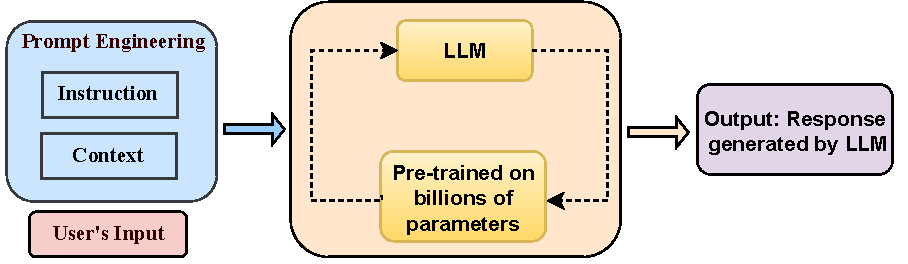
\includegraphics[width =0.50\textwidth, height=3cm]{ijcai-review-page-4.drawio.pdf}\hfill
     % \includegraphics[width=1\textwidth, height=4cm]{IJCAI-review-Page-4.drawio.pdf}
     \caption{Visual breakdown of prompt engineering components: LLMs trained on extensive data, instruction and context as pivotal elements shaping the prompt, and a user input interface.}
  % \caption{Overview of the Prompt Engineering}
  \label{fig:proposedfedbndp}
\end{figure}


\section{Introduction}
Prompt engineering has emerged as a crucial technique for enhancing the capabilities of pre-trained large language models (LLMs) and vision-language models (VLMs). It involves strategically designing task-specific instructions, referred to as prompts, to guide model output without altering parameters. The significance of prompt engineering is especially evident in its transformative impact on the adaptability of LLMs and VLMs. By offering a mechanism to fine-tune model outputs through carefully crafted instructions, prompt engineering enables these models to excel across diverse tasks and domains. This adaptability is different from traditional paradigms, where model retraining or extensive fine-tuning is often required for task-specific performance. This is the transformative promise of prompt engineering, pushing the boundaries of AI and opening doors to a future brimming with possibilities. In an ever-evolving landscape, ongoing research consistently reveals innovative approaches and applications within prompt engineering. The significance of prompt engineering is underscored by its capacity to steer model responses, enhancing the adaptability and applicability of LLMs across diverse sectors. The landscape of contemporary prompt engineering spans a spectrum of techniques, encompassing foundational methods like zero-shot and few-shot prompting to more intricate approaches such as "chain of code" prompting. The notion of prompt engineering was initially investigated and popularized in the LLMs~\citep{liu2023pre},~\citep{tonmoy2024comprehensive},~\citep{chen2023unleashing} later extended to VLMs~\citep{wu2023visual},~\citep{bahng2022exploring}. 
% Despite ample literature on prompt engineering in both LLMs and VLMs, a noticeable gap persists, specifically in a systematic overview of application-centric prompt engineering techniques. Given the recent advancements in prompt engineering, a comprehensive survey is essential for a nuanced understanding of applications and progressions in contemporary research. 
% This survey paper aims to provide a comprehensive exploration of prompt engineering techniques, categorizing them based on application areas. Through a systematic overview, we delve into the nuances of various latest prompting methods, their applications, and the datasets employed. 
% This paper gains importance by systematically consolidating and organizing more than 30 prompting diverse techniques into a comprehensive taxonomy.
Despite the extensive literature on prompt engineering within both LLMs and VLMs, a notable gap remains, particularly concerning a systematic overview of application-centric prompt engineering techniques. With recent strides in prompt engineering, there is a pressing need for a comprehensive survey that offers a nuanced understanding of applications and advancements in contemporary research. This survey dives deep into the ever-evolving landscape of prompt engineering, analyzing over 41 distinct techniques categorized by their diverse applications. Employing a systematic review approach, we meticulously delve into the intricacies of diverse cutting-edge prompting methods. Our examination encompasses their applications, the language models utilized, and the datasets subjected to experimentation, providing a detailed and nuanced analysis of the evolving landscape of prompt engineering. Additionally, we discuss the pros and cons of these techniques, offering insights into their comparative efficacy.
% We unveil a comprehensive taxonomy diagram that sheds light on how these techniques navigate the vast terrain of LLM capabilities (see Fig.~\ref{fig:lit_surv}) and a table summarizes the dataset and employed models(see Table~\ref{table}). 
We present a comprehensive taxonomy diagram that illustrates how these techniques navigate the vast landscape of LLM capabilities (see Fig.\ref{fig:lit_surv}) and provide a table summarizing the datasets, employed models, and evaluation metrics (see Table\ref{table}). From language generation and question answering to code creation and reasoning tasks, prompt engineering empowers the LLMs into performing feats we never thought possible. By bridging the existing gap in the literature, this survey aims to serve as a valuable resource for researchers and practitioners, offering insights into the latest developments and facilitating a deeper understanding of the evolving landscape of prompt engineering. The structure of the paper is organized as follows: Section 2 presents the prompt engineering techniques from both basic to advanced by categorizing application-area and Section 3 provides a conclusion along with considerations for future research endeavors. 

% This survey paper endeavors to offer a comprehensive exploration of prompt engineering techniques, with a meticulous categorization based on application areas. 



% Additionally, we discuss the pros and cons of these techniques, offering insights into their comparative efficacy. Our survey contributes to bridging the existing knowledge gap and serves as a valuable resource for researchers, practitioners, and enthusiasts navigating the evolving landscape of prompt engineering.


% [ayush]
% we conduct the first survey of recent progress in reasoning with language model prompting. We first give some preliminaries on this direction (§2) and then
% propose to organize relevant works by taxonomy (§3). We further provide in-depth comparisons with discussion for insights (§4). To facilitate beginners who are interested in this field, we highlight some
% open resources (§5) as well as potential future directions (§6).
% discusses the broader applications of prompt engineering across various domains.



% This is unlike traditional approaches that require extensive model retraining or fine-tuning. Prompt engineering unlocks the adaptability of LLMs and VLMs, allowing them to excel at diverse capabilities just through well-designed prompts. More importantly, it enables LLMs and VLMs to rapidly acquire new skills and knowledge by prompting, showcasing their few-shot learning potential.

% Prompt engineering has emerged as a pivotal discipline in the realm of large pre-trained models, enhancing the capabilities of both Large Language Models (LLMs) and Vision Language Models (VLMs). At its core, prompt engineering involves the strategic design and implementation of task-specific cues, known as prompts, to guide the output of these large models. This innovative approach enables LLMs and VLMs to make predictions based solely on prompts, without necessitating the modification of model parameters.
% As we delve into the intricacies of prompt engineering, it becomes evident that its importance lies not only in streamlining model integration into real-world applications but also in providing a versatile and efficient means of leveraging pre-trained models. 

% In contrast to conventional approaches, prompt engineering represents a more agile and resource-efficient solution. Whether prompts are manually curated as natural language instructions or automatically generated as vector representations, they serve as powerful conduits for channeling model behavior. This paradigm shift not only enhances the flexibility of large pre-trained models but also accelerates their deployment in practical scenarios. [cg]


% PROMPT engineering is an approach to adapting a large pretrained model, also known as a foundation model, to new tasks by augmenting the model input with task-specific hints. Specifically, the model’s input is augmented by an additional part, called prompt, which could be manually created natural
% language instructions [4], automated generated natural language
% instructions [5], or automated generated vector representations [6].
% The natural language instructions have been also referred to as discrete prompts or hard prompts, while the vector representations are called continuous prompts or soft prompts.

% Prompt engineering has indeed co-appeared and gained prominence with the emergence of large pre-trained models and together led to a paradigm shift in machine learning (ML). 

% The traditional paradigm requires labeling a considerable amount of data and
% then training a task-specific ML model from scratch or finetuning a pre-trained large model. The model’s performance heavily relies on the quality and amount of labeled data, which can be resource-intensive to acquire. Besides, the traditional paradigm requires tuning the model’s parameters to some extent, i.e., entire parameters in the case of training an ML model from scratch or fully fine-tuning a pre-trained model and partial parameters in the
% case of parameter-efficient finetuning. This limits the extensibility
% of an ML model and requires a specific model copy for each task. 


% Recently, prompting a pre-trained large model to adapt it
% for specific tasks has become a new trend. The key idea of
% prompt engineering is to provide hints along with input to guide
% a pre-trained model for solving a new task using its existing
% knowledge. If the hints are human-interpretable natural language
% (hard prompts), the related studies have been referred to as InContext Learning [7], which enable the model to learn from task
% instructions, demonstrations with a few examples, or supporting
% information in the context. Also, the hints could be continuous
% vector representations (soft prompts). The related work has been
% referred to as Prompt-Tuning [6], which optimizes prompts directly in the embedding space of the model.


% Compared to the traditional paradigm, prompt engineering
% has multiple advantages. Firstly, it requires a few labeled data
% to adapt a pre-trained model to new tasks, which greatly reduces
% the effort of human supervision and computation resource for finetuning. Secondly, prompt engineering enables a pre-trained model to perform predictions on new tasks solely based on the prompt without updating any of the model’s parameters, allowing serving a large scale of downstream tasks using the same model. 
% This makes it possible to apply large-scale pre-trained models for real world applications. 



% However, there lacks a comprehensive survey to summarize the recent progress in this field. Mogadala et al. [2021] mainly reviews existing V-L tasks, datasets, and traditional solutions but rarely introduce V-L pre-training methods. Ruan and Jin [2022] focus on Video-Language PTMs instead
% of Vision-Language PTMs. Different from them, our survey
% aims to present a thorough review of VL-PTMs, which summarizes recent research progress and provides pointers to related research. We present the recent mainstream VL-PTMs in Table 1.
% Basically, there are three steps to pre-train a VL-PTM: 1) encode images and texts into latent representations preserving
% their semantics (Section 2); 2) design a performant architecture to model the interaction between two modalities (Section 3); and 3) devise effective pre-training tasks to train the
% VL-PTMs (Section 4). After learning universal vision and
% language features, VL-PTMs can be fine-tuned on various
% downstream V-L tasks (Section 5). 

% Finally, we conclude this survey and point out some promising research directions in Section 6. 



\begin{figure*}[ht!]
  \centering
  \resizebox{0.85\textwidth}{!}{
    \begin{forest}
      forked edges,
      for tree={
        grow=east,
        reversed=true,
        anchor=base west,
        parent anchor=east,
        child anchor=west,
        base=center,
        font=\large,
        rectangle,
        draw=hidden-draw,
        rounded corners,
        align=center,
        text centered,
        minimum width=5em,
        edge+={darkgray, line width=1pt},
        s sep=3pt,
        inner xsep=2pt,
        inner ysep=3pt,
        line width=0.8pt,
        ver/.style={rotate=90, child anchor=north, parent anchor=south, anchor=center},
      },
      where level=1{text width=15em,font=\normalsize,}{},
      where level=2{text width=14em,font=\normalsize,}{},
      where level=3{minimum width=10em,font=\normalsize,}{},
      where level=4{text width=26em,font=\normalsize,}{},
      where level=5{text width=20em,font=\normalsize,}{},
      [
        \textbf{Prompt Engineering}, for tree={fill=paired-light-red!80}, text width=14em
        [
              \textbf{New Tasks Without Extensive}\\ \textbf{Training} \S\ref{newtask}, for tree={fill=red!50}, text width=18em
              [
                \textbf{Zero-shot Prompting} \citep{radford2019language}, for tree={fill=pg58},text width=28em
              ]
              [
                \textbf{Few-shot Prompting} \citep{brown2020language}, for tree={fill=pg58},text width=28em
              ]
        ]
        [
            \textbf{Reasoning and Logic} \S\ref{ral}, for tree={fill=green!50}, text width=18em
            [
            \textbf{Chain-of-Thought (CoT) Prompting}~\citep{wei2022chain} , for tree={fill=bg4},text width=28em
            ]
            [
            \textbf{Automatic Chain-of-Thought (Auto-CoT)}~\citep{zhang2022automatic} , for tree={fill=bg4},text width=28em
            ]
            [
            \textbf{Self-Consistency}~\citep{wang2022self} , for tree={fill=bg4},text width=28em
            ]
            [
            \textbf{Logical CoT (LogiCoT) Prompting}~\citep{zhao2023enhancing} , for tree={fill=bg4},text width=28em
            ]p
            [
            \textbf{Chain-of-Symbol (CoS) Prompting}~\citep{hu2023chainofsymbol} , for tree={fill=bg4},text width=28em
            ]
            [
            \textbf{Tree-of-Thoughts (ToT) Prompting}~\citep{yao2023tree} , for tree={fill=bg4},text width=28em
            ]
            [
            \textbf{Graph-of-Thought (GoT) Prompting}~\citep{yao2023beyond} , for tree={fill=bg4},text width=28em
            ]
            [
            \textbf{System 2 Attention Prompting}~\citep{weston2023system} , for tree={fill=bg4},text width=28em
            ]
            [
            \textbf{Thread of Thought (ThoT) Prompting}~\citep{zhou2023thread} , for tree={fill=bg4},text width=28em
            ]
            [
            \textbf{Chain of Table Prompting}~\citep{wang2024chainoftable} , for tree={fill=bg4},text width=28em
            ]
            [
            \textbf{ Self-Refine Prompting}~\citep{madaan2023selfrefine} , for tree={fill=bg4},text width=28em
            ] 
            [
            \textbf{ Code Prompting}~\citep{puerto2024codepromptingelicitsconditional} , for tree={fill=bg4},text width=28em
            ]
            [
            \textbf{Self-Harmonized CoT (ECHO) Prompting}~\citep{mekala2024echopromptinstructingmodelrephrase} , for tree={fill=bg4},text width=28em
            ]
            [
            \textbf{Logic-of-Thought Prompting}~\citep{liu2024logicofthoughtinjectinglogiccontexts} , for tree={fill=bg4},text width=28em
            ]
            [
            \textbf{ Instance-adaptive Prompting (IAP) }~\citep{yuan2024instanceadaptivezeroshotchainofthoughtprompting} , for tree={fill=bg4},text width=28em
            ]
            [
            \textbf{ End-to End DAG-Path (EEDP) Prompting }~\citep{yuan2024instanceadaptivezeroshotchainofthoughtprompting} , for tree={fill=bg4},text width=28em
            ]
            [
            \textbf{ Layer-of-Thoughts (LoT) }~\citep{fungwacharakorn2024layerofthoughtspromptinglotleveraging} , for tree={fill=bg4},text width=28em
            ]
            [
            \textbf{ Narrative-of-Thought (NoT) Prompting}~\citep{zhang2024narrativeofthoughtimprovingtemporalreasoning} , for tree={fill=bg4},text width=28em
            ]
            [
             \textbf{ Buffer of Thoughts (BoT) Prompting}~\citep{yang2024buffer} , for tree={fill=bg4},text width=28em
            ]
            [
            \textbf{ Contrastive Denoising with Noisy Chain-of-Thought (CD-CoT)}\\ \textbf{Prompting}~\citep{NEURIPS2024_dfaa29ed} , for tree={fill=bg4},text width=28em
            ]
            [
            \textbf{Reverse Chain-of-Thought (R-CoT) Prompting}~\citep{deng2024rcotreversechainofthoughtproblem} , for tree={fill=bg4},text width=28em
            ]
            [
            \textbf{Chain of Draft (CoD) Prompting}~\citep{xu2025chaindraftthinkingfaster} , for tree={fill=bg4},text width=28em
            ]   
        ]
        [
            \textbf{Reduce Hallucination} \S\ref{rh}, for tree={fill=lime!50}, text width=18em
            [
            \textbf{Retrieval Augmented Generation (RAG)}~\citep{lewis2020retrieval} , for tree={fill=bg32},text width=28em
            ]
            [
            \textbf{ReAct Prompting}~\citep{yao2022react} , for tree={fill=bg32},text width=28em
            ]
            [
            \textbf{Chain-of-Verification (CoVe)}~\citep{dhuliawala2023chain} , for tree={fill=bg32},text width=28em
            ]
            [
            \textbf{Chain-of-Note (CoN) Prompting}~\citep{yu2023chainofnote} , for tree={fill=bg32},text width=28em
            ]
            [
            \textbf{Chain-of-Knowledge (CoK) Prompting}~\citep{li2023chainofknowledge} , for tree={fill=bg32},text width=28em
            ]
        ]
        [
            \textbf{User Interaction} \S\ref{ui}, for tree={fill=bg25}, text width=18em
            [
            \textbf{Active-Prompt}~\citep{diao2023active} , for tree={fill=bg8},text width=28em
            ]
        ]
        [
            \textbf{Fine-Tuning and Optimization} \S\ref{fto}, for tree={fill=purple!50}, text width=18em
            [
            \textbf{Automatic Prompt Engineer (APE)}~\citep{zhou2022large} , for tree={fill=bg10},text width=28em
            ]
        ]
        [
            \textbf{Knowledge-Based Reasoning and} \\ \textbf{Generation}\S\ref{kbrg}, for tree={fill=bg34}, text width=18em
            [
            \textbf{Automatic Reasoning}\\ \textbf{and Tool-use (ART)}~\citep{paranjape2023art} , for tree={fill=bg37},text width=28em
            ]
        ]
        [
            \textbf{Improving Consistency} \\ \textbf{and Coherence} \S\ref{icc}, for tree={fill=bg33}, text width=18em
            [
            \textbf{Contrastive Chain-of-Thought} \\ \textbf{Prompting (CCoT)}~\citep{chia2023contrastive} , for tree={fill=pink!50},text width=28em
            ]
        ]
        [
            \textbf{Managing Emotions and Tone} \S\ref{met}, for tree={fill=bg40}, text width=18em
            [
            \textbf{Emotion Prompting}~\citep{li2023large} , for tree={fill=paired-light-yellow!50},text width=28em
            ]
        ]
        [
          \textbf{Code Generation and Execution} \S\ref{cge}, for tree={fill=cyan!50}, text width=18em
          % [ \textbf{Handles only Images}, for tree={fill=bg22}, text width=13.5em             
              [
                \textbf{Scratchpad Prompting}~\citep{nye2021show} , for tree={fill=bg16},text width=28em
              ]
              [
                \textbf{Program of Thoughts (PoT) Prompting}~\citep{chen2022program},text width=28em, for tree={fill=bg16}
                ]
              [
                \textbf{Structured Chain-of-Thought}\\ \textbf{(SCoT) Prompting}~  \citep{li2023structured},text width=28em, for tree={fill=bg16}
                ]
             [
                \textbf{Chain of Code (CoC) Prompting}~\citep{li2023chain},text width=28em, for tree={fill=bg16}
                ]
        ]
        [
            \textbf{Optimization and Efficiency} \S\ref{oe}, for tree={fill=bg15}, text width=18em
            [
                \textbf{Optimization by Prompting}~\citep{yang2023large}, text width=28em, for tree={fill=bg7}
            ]
        ]
        [
            \textbf{Understanding User Intent} \S\ref{uui}, for tree={fill=blue!50}, text width=18em
            [
                \textbf{Rephrase and Respond (RaR) Prompting}~\citep{deng2023rephrase}, text width=28em, for tree={fill=bg38} 
            ]
        ]
        [
            \textbf{Metacognition and Self-Reflection} \S\ref{mas}, for tree={fill=bg1}, text width=18em
            [
                \textbf{Take a Step Back Prompting}~\citep{zheng2023take}, text width=28em, for tree={fill=bg36}
            ]
        ]
      ]
    \end{forest}
    }
  \caption{Taxonomy of prompt engineering techniques in LLMs, organized around application domains, providing a nuanced framework for customizing prompts across diverse contexts.}
  \label{fig:lit_surv}
\end{figure*}




\section{Prompt Engineering}
In this section, we have organized prompt engineering techniques according to their application areas and provided a concise overview of the evolution of prompting techniques, spanning from zero-shot prompting to the latest advancements. 
% up to the completion date of our survey paper on January 31, 2024.


\subsection{New Tasks Without Extensive Training}
\label{newtask}
\subsubsection{Zero-Shot Prompting} 
\label{zero}
Zero-shot prompting offers a paradigm shift in leveraging large LLMs. This technique removes the need for extensive training data, instead relying on carefully crafted prompts that guide the model toward novel tasks~\citep{radford2019language}. Specifically, the model receives a task description in the prompt but lacks labeled data for training on specific input-output mappings. The model then leverages its pre-existing knowledge to generate predictions based on the given prompt for the new task.
% For instance, in sentiment classification, the model could be prompted to identify emotions in sentences, even without prior exposure to labeled instances associating sentences with emotions.  

% Zero-shot prompting is when a model is given a task without prior training examples. Specifically, the model receives a task description in the prompt but lacks \textbf{labeled data for training on specific input-output mappings.} The model then leverages its pre-existing knowledge to generate predictions based on the given prompt for the new task. To illustrate, in the context of sentiment classification, the model might be prompted to identify emotions in sentences, even though it has not been exposed to prior training instances associating sentences with emotions. This approach allows the model to extend its capabilities to new tasks and domains without requiring extensive labeled datasets for each potential task.

% % Example: \\
% \textbf{Prompt:} Classify the text into neutral, negative, or positive. Text: "I love the sunny weather." \\
% Sentiment:\\
% \textbf{Output:} Positive. \\

\subsubsection{Few-Shot Prompting}
\label{few}
Few-shot prompting provides models with a few input-output examples to induce an understanding of a given task, unlike zero-shot prompting, where no examples are supplied~\citep{brown2020language}. Providing even a few high-quality examples has improved model performance on complex tasks compared to no demonstration. However, few-shot prompting requires additional tokens to include the examples, which may become prohibitive for longer text inputs. Moreover, the selection and composition of prompt examples can significantly influence model behavior, and biases like favoring frequent words may still affect few-shot results. While few-shot prompting enhances capabilities for complex tasks, especially among large pre-trained models like GPT-3, careful prompt engineering is critical to achieve optimal performance and mitigate unintended model biases. 

% Example:

% \textbf{Prompt:} For sentiment analysis\\
% Positive: "I enjoyed the movie." \\
% Negative: "The restaurant service was terrible." \\
% Neutral: "The weather today is okay."\\
% \textcolor{blue}{“The book is fascinating," and ask it to predict the sentiment.} \\

\subsection{Reasoning and Logic}
\label{ral}
\subsubsection{Chain-of-Thought (CoT) Prompting} 
\label{cot}
LLMs often stumble in the face of complex reasoning, limiting their potential. Aiming to bridge this gap, \cite{wei2022chain} introduced Chain-of-Thought (CoT) prompting as a technique to prompt LLMs in a way that facilitates coherent and step-by-step reasoning processes. The primary contribution lies in the proposal and exploration of CoT prompting, demonstrating its effectiveness in eliciting more structured and thoughtful responses from LLMs compared to traditional prompts. Through a series of experiments, the authors showcase the distinctive qualities of CoT prompting, emphasizing its ability to guide LLMs through a logical reasoning chain. This results in responses that reflect a deeper understanding of the given prompts. For example, the prompt would show the reasoning process and final answer for a multi-step math word problem and mimic how humans break down problems into logical intermediate steps. The authors achieved state-of-the-art performance in math and commonsense reasoning benchmarks by utilizing CoT prompts for PaLM 540B, achieving an accuracy of 90.2\%.

% The authors showed state-of-the-art math and commonsense reasoning benchmark performance by prompting large models like PaLM with just a few CoT examples, outperforming even fine-tuned GPT-3.


\subsubsection{Automatic Chain-of-Thought (Auto-CoT) Prompting}
\label{auto-cot}
Manual creation of high-quality CoT examples is both time-consuming and suboptimal.~\cite{zhang2022automatic} introduced Auto-CoT to automatically instruct LLMs with a "Let's think step-by-step" prompt to generate reasoning chains. Recognizing the possibility of errors in individually generated chains, Auto-CoT enhances robustness through diverse sampling. It samples various questions and generates multiple distinct reasoning chains for each, forming a final set of demonstrations. This automated diverse sampling minimizes errors and enhances few-shot learning, eliminating the need for labor-intensive manual creation of reasoning chains. Auto-CoT demonstrated enhanced performance, surpassing the CoT paradigm with average accuracy improvements of 1.33\% and 1.5\% on arithmetic and symbolic reasoning tasks, respectively, employing GPT-3.

% Auto-CoT improved average accuracy by 1.33\% and 1.5\% over the CoT paradigm on arithmetic and symbolic reasoning tasks with GPT-3, respectively.
% Auto-CoT improved average accuracy by 1.33\% and 1.5\% over the CoT paradigm, respectively. 

\subsubsection{Self-Consistency}
\label{selfcon}
\cite{wang2022self} introduced self-consistency, a decoding strategy enhancing reasoning performance compared to greedy decoding in CoT prompting. For complex reasoning tasks with multiple valid paths, self-consistency generates diverse reasoning chains by sampling from the language model's decoder. It then identifies the most consistent final answer by marginalizing these sampled chains. This approach capitalizes on the observation that problems requiring thoughtful analysis often entail greater reasoning diversity, leading to a solution. The combination of self-consistency and chain-of-thought prompting results in significant accuracy improvements across various benchmarks, such as 17.9\% on GSM8K, 11.0\% on SVAMP, 12.2\% on AQuA, 6.4\% on StrategyQA, and 3.9\% on ARC-challenge compared to the baseline chain-of-thought prompting.


\subsubsection{Logical Chain-of-Thought (LogiCoT) Prompting}

\textls[-10]{The ability to perform logical reasoning is critical for LLMs to solve complex, multi-step problems across diverse domains. Existing methods, like CoT prompting, encourage step-by-step reasoning but lack effective verification mechanisms.  \cite{zhao2023enhancing} proposes a Logical Chain-of-Thought (LogiCoT) prompting, a neurosymbolic framework that leverages principles from symbolic logic to enhance reasoning in a coherent and structured manner. Specifically, LogiCoT applies the concept of reductio ad absurdum to verify each step of reasoning generated by the model and provide targeted feedback to revise incorrect steps. LogiCoT can reduce logical errors and hallucinations through a think-verify-revise loop. 
Experimenting with Vicuna-33b and GPT-4, the findings underscore LogiCoT's notable enhancement of reasoning abilities, exhibiting improvements of 0.16\% and 1.42\% on the GSM8K dataset and 3.15\% and 2.75\% on the AQuA dataset compared to CoT, respectively.}


% Experimental results, utilizing datasets like GSM8K and AQuA across models from Vicuna-7b to GPT-4, underscore LogiCoT's ability to significantly enhance reasoning capabilities, with 0.16\% and 1.42\% improvements compared to CoT.


% Experimenting with datasets such as GSM8K and AQuA across various models from Vicuna-7b to GPT-4, the findings emphasize LogiCoT's capacity to boost reasoning abilities, showcasing improvements of 0.16\% and 1.42\% compared to CoT.

% Experimenting with datasets such as GSM8K and AQuA on Vicuna-33b and GPT-4, the findings emphasize LogiCoT's capacity to notably boost reasoning abilities, with improvements of 0.16\% and 1.42\% compared to CoT, respectively.

% Experimenting with Vicuna-33b and GPT-4, the findings emphasize LogiCoT's capacity to notably boost reasoning abilities, with improvements of 0.16\% and 1.42\% on GSM8K and 3.15\% and 2.75\% on AQuA dataset compared to CoT, respectively.

% Through experiments with datasets like GSM8K and AQuA, spanning models from Vicuna-7b to GPT-4, the results highlight that LogiCoT significantly improves reasoning abilities, particularly as the model scale increases.


\subsubsection{Chain-of-Symbol (CoS) Prompting}
\label{cos}
\textls[0]{LLMs often struggle with tasks involving complex spatial relationships due to their reliance on natural language, which is susceptible to ambiguity and biases. To overcome this limitation, \cite{hu2023chainofsymbol} introduced CoS, employing condensed symbols instead of natural language. CoS provides distinct advantages: clear and concise prompts, heightened spatial reasoning for LLMs, and improved human interpretability. CoS suffers from challenges such as scalability, generalizability, integration with other techniques, and interpretability of LLM reasoning based on symbols. Notably, the implementation of CoS significantly elevates ChatGPT's performance, boosting accuracy from 31.8\% to an impressive 92.6\% on Brick World tasks. Moreover, CoS achieves up to a 65.8\% reduction in prompt tokens, streamlining the process while maintaining high accuracy.}






% Phase 1: question clustering: categorize questions from a provided dataset into several clusters. 

% Phase 2: demonstration sampling: choose a representative question from each cluster and produce its reasoning chain utilizing Zero-Shot-CoT alongside straightforward heuristics. 
% These heuristics may involve factors like question length (e.g., 60 tokens) and the number of steps in rationale (e.g., 5 reasoning steps), aiming to prompt the model to employ clear and precise demonstrations.[paraphrase]\\
% \textbf{Prompt:}\\
% Q: Ryan bought video games online. He bought 4 action games and 2 adventure games. Each game came with a map and had 5 levels. How many total levels did Ryan buy?\\
% A: Let's think step-by-step:\\
% Ryan bought 4 action games. Each action game has 5 levels. So he got 4 * 5 = 20 levels from the action games. Ryan also bought 2 adventure games. Each adventure game has 5 levels. So he got 2 * 5 = 10 levels from the adventure games. In total Ryan bought 20 + 10 = 30 levels. Therefore, the total number of levels Ryan bought is 30.




% Early results highlight improved complex reasoning abilities in CoT-prompted language models, reflecting deeper principles of diverse deliberative reasoning paths.


% \textbf{Prompt:}\\
% Q: In the garden, there are 8 sunflowers. If 4 more sunflowers bloom, how many sunflowers are there in the garden?\\
% A: Initially, there are 8 sunflowers in the garden. As 4 more bloom, the total number of sunflowers becomes 8 + 4 = 12. The answer is 12.\\
% Q: When I was 10, my brother was half my age. Now I’m 45, how old is my brother?\\
% A: Output 1: When I was 10, my brother was half my age, so he was 5. Now I am 45, so he is 45 - 5 = 40. The answer is 40.\\
% Output 2: When the narrator was 10, his brother was half his age, which is 5. Now that the narrator is 45, his brother would be 45 - 5 = 40 years old. The answer is 40.\\
% Output 3: When I was 10, my brother was half my age, so he was 5. Now I am 45, so he is 45/2 = 22.5.\\
% The answer is 40. The answer which remains consistent in all the outputs will be the final answer.

\subsubsection{Tree-of-Thoughts (ToT) Prompting}
\label{tot}
\textls[-10]{\cite{yao2023tree} and ~\cite{long2023large} proposed the Tree-of-Thoughts (ToT) framework to enhance prompting capabilities for complex tasks requiring exploration and look-ahead reasoning. ToT extends CoT prompting by managing a tree structure of intermediate reasoning steps, known as "thoughts". Each thought represents a coherent language sequence moving toward the final solution. This structure allows language models to deliberately reason by assessing the progress generated by thoughts in solving the problem. ToT integrates the model's abilities to produce and evaluate thoughts with search algorithms like breadth-first or depth-first search. This enables systematic exploration among reasoning chains, with a look-ahead to expand promising directions and to backtrack when solutions are incorrect. ToT excelled in the Game of 24 tasks, achieving a 74\% success rate compared to CoT's 4\%. Additionally, in word-level tasks, ToT outperformed CoT with a 60\% success rate versus 16\%.}

% \textbf{Prompt:}\\
% Sally is in the bedroom. She walks to the kitchen carrying a bowl. She puts an orange in the bowl and carries it to the living room. She turns the bowl upside down on the couch, then walks to the backyard. She puts the bowl down in the backyard then walks to the garage. Where is the orange?
% Here's the prompt I used:
% Imagine three different experts are answering this question.
% All experts will write down 1 step of their thinking,
% then share it with the group.
% Then all experts will go on to the next step, etc.
% If any expert realises they're wrong at any point then they leave.
% The question is...
% Output:

% Expert 1: Sally put the orange in the bowl in the kitchen.

% Expert 2: Sally carried the bowl with the orange to the living room.

% Expert 3: Sally flipped the bowl upside down on the couch, spilling out the orange.

% Expert 1: I agree, when Sally flipped the bowl, the orange spilled onto the couch.

% Expert 2: Yes, the orange ended up on the couch in the living room.

% Since the experts agree the orange spilled onto the couch when Sally flipped the bowl, they do not need to discuss Sally going to the backyard and garage afterward.


\subsubsection{Graph-of-Thoughts (GoT) Prompting}
\label{got}
\textls[-10]{The inherent non-linear nature of human thought processes challenges the conventional sequential approach of CoT prompting.~\cite{yao2023beyond} introduced the "Graph of Thoughts" prompting, a graph-based framework advancing traditional sequential methods to better align with the non-linear characteristics of human thinking. This framework permits dynamic interplay, backtracking, and evaluation of ideas, allowing the aggregation and combination of thoughts from various branches, departing from the linear structure of the tree of thoughts. The key contributions encompass modeling the reasoning process as a directed graph, offering a modular architecture with diverse transformation operations. The framework is presented as a versatile and dynamic approach to language model prompting, capturing the intricacies of human thought processes and enhancing model capabilities. The GoT reasoning model demonstrates substantial gains over the CoT baseline, improving accuracy by 3.41\% with T5-base and 5.08\% with T5-large on GSM8K. It also boosts accuracy over the state-of-the-art Multimodal-CoT by 6.63\% using T5-base and 1.09\% with T5-large on ScienceQA.}

% The integration of LLMs in NLP tasks prompted researchers to explore the CoT concept for aiding LLMs in complex reasoning tasks by generating intermediate steps. However, the inherent non-linear nature of human thought processes challenges the conventional sequential approach of CoT.~\cite{yao2023beyond} have introduced a groundbreaking paradigm in language model prompting, advancing beyond traditional sequential methods to better align with the non-linear characteristics of human thinking. Their paper introduces a graph-based framework, a notable evolution from the "Tree of Thoughts" concept. This framework permits dynamic interplay, backtracking, and evaluation of ideas, allowing the aggregation and combination of thoughts from various branches, departing from the linear structure of the tree of thoughts. Key contributions encompass modeling the reasoning process as a directed graph, offering a modular architecture with diverse transformation operations. The paper demonstrates the framework's efficacy in decomposable problems, introducing the "volume of thoughts" metric to quantify the incorporation of intermediary thoughts for a more refined solution. The graph of thoughts framework is presented as a versatile and dynamic approach to language model prompting, capturing the intricacies of human thought processes and enhancing model capabilities. The accompanying code provides additional insights into the modular architecture. In summary, the paper marks a substantial advancement in language model prompting, introducing a flexible, contextually relevant graph-based framework that holds promise for future NLP applications.

\subsubsection{System 2 Attention (S2A) Prompting}
\label{s2a}
\textls[-10]{The soft attention mechanism in Transformer-based LLMs is prone to incorporating irrelevant context information, impacting token generation adversely. To address this,~\cite{weston2023system} proposed System 2 Attention (S2A), utilizing the reasoning abilities of LLMs to selectively attend to relevant portions by regenerating the input context. S2A employs a two-step process to enhance attention and response quality by employing context regeneration and response generation with refined context. The effectiveness of S2A is evaluated across various tasks, including factual QA, long-form generation, and math word problems. In factual QA, S2A attains an accuracy of 80.3\%, demonstrating a substantial enhancement in factuality. In long-form generation, it improves objectivity and receives a score of 3.82 out of 5.}

\subsubsection{Thread of Thought (ThoT) Prompting}
\label{thot}
\textls[-10]{\cite{zhou2023thread} presented Thread of Thought (ThoT), a prompting technique designed to enhance the reasoning abilities of LLMs within chaotic contexts. ThoT, inspired by human cognition, systematically examines extensive contexts into manageable segments for incremental analysis, employing a two-phase approach where the LLM first summarizes and examines each segment before refining the information for a final response. ThoT's flexibility shines as a versatile "plug-and-play" module, enhancing reasoning across different models and prompting methods. Evaluations on question answering and conversation datasets reveal substantial performance improvements of 47.20\% and 17.8\%, respectively, especially in chaotic contexts.}

% ThoT's flexibility shines as a versatile "plug-and-play" module, enhancing reasoning across different models and prompting methods. Evaluations on question answering and conversation datasets reveal substantial performance improvements of 47.20\% and 17.8\%, respectively, especially in chaotic contexts.

\subsubsection{Chain-of-Table Prompting}
\label{cotp}
\textls[-10]{Approaches like CoT, PoT, and ToT represent reasoning steps through free-form text or code, which face challenges when dealing with intricate table scenarios. The study by~\cite{wang2024chainoftable} introduced a pioneering prompting technique named Chain-of-Table. This method uses step-by-step tabular reasoning by dynamically generating and executing common SQL/DataFrame operations on tables. The iterative nature of this process enhances intermediate results, empowering LLMs to make predictions through logically visualized reasoning chains. Significantly, Chain-of-Table consistently improves the performance of two benchmark tabular datasets by 8.69\% on TabFact and 6.72\% on WikiTQ, respectively.}
% Understanding tabular data with language models can benefit various downstream tasks, such as table-based fact verification, and table-based question answering. Distinct from pure text, tables deliver rich information through the interaction between rows and columns in the tabular structure, which enhances the data capacity but also increases the difficulty for language models to understand them. Thus, reasoning over the tabular data is an important direction in natural language processing and attracts increasing attention from both academia and industry.
% In recent years, several approaches have been suggested to tackle the problem of table understanding by training language models. One common direction is to add specialized embedding layers or attention mechanisms into language models and pre-train the models by recovering table cells or segments.
% Another direction is to synthesize SQL query-response pairs and pre-train an encoderdecoder model as a neural SQL executor.
% However, these approaches like COT, Least-to-Most, Program-of-Thought and Tree-of-Thought often represent reasoning steps in free-form text or code, which are not ideally suited for addressing scenarios involving complex tables.
% Conversely, our proposed CHAIN-OF-TABLE consistently improves End-to-End QA performance by 8.69% on TabFact and 6.72% on WikiTQ when implemented with PaLM 2.
%[] We introduce CHAIN-OF-TABLE, a method in which we perform step-by-step reasoning through tabular operations, creating a chain of tables. Each table in the chain represents the intermediate reasoning results, transformed by the corresponding tabular operations.
% Analyzing tabular data with language models is valuable for tasks like fact verification and question answering. The structured nature of tables provides rich information, but it poses challenges for language models. Reasoning over tabular data is a crucial focus in natural language processing, gaining attention from academia and industry due to its potential applications in enhancing information extraction and understanding.
% Recent approaches for table understanding in language models involve incorporating specialized embeddings or attention mechanisms, with pre-training focusing on tasks like recovering table cells. Another direction utilizes the synthesis of SQL query-response pairs, employing an encoder-decoder model as a neural SQL executor for pre-training.
% methods like COT, Least-to-Most, Program-of-Thought, and Tree-of-Thought typically depict reasoning steps using free-form text or code, which may not be well-suited for handling complex table scenarios.
% CHAIN-OF-TABLE is proposed, conducting step-by-step reasoning through tabular operations to form a chain of tables. The tables in the chain represent the transformed tables by the tabular operations, reflecting the intermediate reasoning results.
% \vspace{2mm}
\subsubsection{Self-Refine Prompting}\label{Self-refine}
\noindent \textls[-10]{Self-Refine prompting, proposed by ~\cite{madaan2023selfrefine}, enhances LLM performance by iteratively refining outputs through self-generated feedback, mimicking human revision. While LLMs can handle a wide range of tasks, they often struggle with complex objectives, ambiguous goals, or multi-step reasoning, leading to initial responses with inaccuracies or flawed logic. Inspired by human iterative refinement, Self-Refine enables LLMs to improve their outputs through a structured three-step process: generating an initial response, prompting the model to critique its own output, and refining the response based on this feedback. This cycle continues until predefined stopping criteria are met, allowing the model to produce more accurate and contextually relevant results. Unlike traditional prompting methods, which rely solely on a single-step response, Self-Refine fosters incremental improvement, making it particularly effective for tasks requiring nuanced reasoning. Experimental results demonstrate significant performance gains, with GPT-4 improving by 8.7 points in code optimization, 13.9 points in code readability, and 21.6 points in sentiment reversal tasks, showcasing its potential to enhance the reasoning and adaptability of LLMs across various domains.}
\subsubsection{Code Prompting}\label{code}
\noindent \textls[-10]{Pre-training on code enhances the reasoning capabilities of LLMs, yet the underlying mechanisms driving this improvement remain poorly understood. To investigate this,~\cite{puerto2024codepromptingelicitsconditional} examines the impact of input representation on LLM reasoning, specifically exploring whether reformulating natural language (NL) problems into code can trigger conditional reasoning abilities. 
This led to the introduction of Code Prompting, a technique that reformulates NL tasks into structured code, enabling direct prompting of text+code LLMs without relying on external code execution. Experiments on three reasoning benchmarks, ConditionalQA, BoardgameQA, and ShARC, demonstrate that code prompts significantly outperform traditional text-based prompts. On average, GPT 3.5 achieved a performance gain of 8.42 F1 score, while Mistral showed an average improvement of 4.22 across the three datasets.}
\subsubsection{Self-Harmonized Chain-of-Thought (ECHO) Prompting}
 \label{ECHO}
% Chain-of-Thought prompting has significantly enhanced the reasoning capabilities of LLMs by decomposing complex problems into intermediate steps. 
% However, fully automated techniques like Auto-CoT which generate demonstrations without human intervention suffer notable drawbacks. They often exhibit misleading similarity, where erroneous reasoning paths are repeatedly generated for similar examples. Moreover, these methods sometimes produce outputs with ineffective diversity, yielding overly varied or irrelevant patterns.
% However, fully automated techniques such as Auto-CoT, which generate demonstrations without human intervention, often suffer from misleading similarity, where incorrect reasoning paths are repeated and ineffective diversity, yielding overly varied or irrelevant patterns. To address these challenges, Jin and Lu (2024) introduced ECHO, a self-harmonized prompting framework that unifies diverse reasoning paths into a coherent, robust pattern.
% ECHO operates in three key stages: (1) Question Clustering, where Sentence-BERT embeddings and k-means clustering group similar questions to identify representative clusters; (2) Demonstration Sampling, which selects a representative question from each cluster and generates its rationale via Zero-Shot-CoT; and (3) Demonstration Unification, where the generated rationales are iteratively refined through a dynamic prompting mechanism to align the diverse reasoning patterns. This process minimizes noise introduced by heterogeneous demonstrations while preserving adaptability. Notably, ECHO outperformed Auto-CoT by an average of 2.8\% across 10 reasoning benchmarks (spanning arithmetic, commonsense, and symbolic tasks), and it maintained performance with 50\% fewer examples—a -0.8\% decline compared to Few-Shot-CoT’s -1.3\% drop. Despite these gains, a gap remains compared to GPT-3.5, attributed to differences in the inherent quality of reasoning rationales.
\noindent While Chain-of-Thought prompting enhances reasoning in LLMs, methods like Auto-CoT, which automate demonstration generation, face challenges from misleading similarity (incorrect rationales in similar examples) and ineffective diversity (irrelevant or overly varied patterns). To address these issues,~\cite{mekala2024echopromptinstructingmodelrephrase} introduced ECHO, a self-harmonized prompting framework that unifies diverse reasoning paths into a coherent pattern, balancing automation with robustness. ECHO operates through three key stages: (1) Question Clustering, where Sentence-BERT embeddings and k-means group questions into clusters; (2) Demonstration Sampling, which selects representative questions from each cluster and generates rationales using Zero-Shot-CoT; and (3) Demonstration Unification, where rationales are iteratively refined using a dynamic prompting mechanism to align reasoning patterns. This process minimizes diversity-induced noise while retaining adaptability. ECHO surpassed Auto-CoT by an average of 2.8\% across 10 reasoning benchmarks (arithmetic, commonsense, symbolic) while demonstrating greater efficiency. It retained performance with 50\% fewer examples, showing only a -0.8\% dip compared to Few-Shot-CoT’s -1.3\% decline. The method also achieved 2.3\% gains over Auto-CoT in Mixtral-8x7B, though it remained behind GPT-3.5, a gap attributed to differences in the quality of reasoning rationales.
\subsubsection{Logic-of-thought Prompting}
\label{LoT}
\noindent \textls[-10]{LLMs often exhibit unfaithful reasoning, where the generated conclusions diverge from the intermediate reasoning steps. Logic-of-Thought prompting~\citep{liu2024logicofthoughtinjectinglogiccontexts} is a neuro‐symbolic framework developed to mitigate this issue by enriching prompts with logical information derived from propositional logic. LoT operates in three phases: (1) Logic Extraction, during which LLMs identify propositions and logical relationships from input texts; (2) Logic Extension, in which a Python-based module applies formal logical laws (e.g., contraposition) to infer additional expressions; and (3) Logic Translation, where the extended logic is rendered back into natural language and appended to the original prompt to ensure contextual fidelity. Moreover, Logic-of-thought is designed to integrate seamlessly with other prompting strategies such as CoT, Self-Consistency, and ToT prompting. Reported evaluations indicate that Logic-of-thought can improve CoT accuracy on the ReClor benchmark by 4.35\%, enhance CoT prompting with Self-Consistency on LogiQA by 5\%, and further boost ToT prompting performance on the ProofWriter dataset by 8\%. Additionally, by preserving natural language representations throughout the process, Logic-of-Thought avoids the symbolic extraction errors that can impair other neuro‐symbolic systems, such as SatLM.}
% LLMs often exhibit unfaithful reasoning, where generated conclusions misaligned with intermediate reasoning steps. Logic-of-thought (LoT) prompting~\cite{liu2024logicofthoughtinjectinglogiccontexts} is a neuro-symbolic framework designed to improve the reasoning fidelity of LLMs. LoT addresses unfaithful reasoning by augmenting prompts with expanded logical information derived from propositional logic. It operates through three key phases: (1) Logic Extraction, where LLMs identify propositions and logical relationships from input contexts; (2) Logic Extension, where a python-based program applies logical laws (e.g., Contraposition) to infer new expressions; and (3) Logic Translation, where extended logic is transformed into natural language and appended to prompts, ensuring contextual consistency.
% LoT integrates seamlessly with other prompting techniques like Chain-of-Thought, Self-Consistency, and Tree-of-Thoughts. The LoT increases Chain-of-Thought’s accuracy on the ReClor benchmark by 4.35 \%. It also elevates Chain-of-Thought with Self-Consistency’s results on LogiQA by 5\% while further enhancing Tree-of-Thoughts’ effectiveness on the ProofWriter dataset by 8\%. By retaining natural language, LoT avoids errors associated with symbolic extraction, outperforming neuro-symbolic baselines like SatLM.
% }
% LLMs excel in many reasoning tasks, they often struggle with precision-recall trade-offs and explainability in complex retrieval scenarios, particularly in domains like legal analysis. Layer-of-Thoughts (LoT) prompting~\cite{fungwacharakorn2024layerofthoughtspromptinglotleveraging} is a hierarchical reasoning framework that improves structured retrieval by leveraging constraint hierarchies. Designed for complex scenarios like legal analysis, LoT organises reasoning into layer thoughts (conceptual stages) and option thoughts (partial solutions), applying sequential layers of constraints to iteratively filter and refine candidate responses. For example, in legal document retrieval, LoT employs three layers: (1) Keyword Filtering Layer (KFL) extracts LLM-generated keywords to filter documents using metrics like at-least-k; (2) Semantic Filtering Layer (SFL) prioritizes documents using multi-level relevance criteria and aggregation metrics; and (3) Final Confirmation Layer (FCL) validates final candidates against the original query through all constraints. LoT combines hard constraints (required) and soft constraints (preferential) for dynamic prioritization and explainable reasoning. It outperformed state-of-the-art models like JNLP on Japanese Civil Law retrieval (F2: 0.835 vs. 0.807) by balancing precision (0.838) and recall (0.839). In German traffic law, it achieved near-perfect recall (0.966), ensuring minimal oversight in critical legal contexts.
\subsubsection{Instance-adaptive Prompting (IAP)}
\label{IAP}
\noindent \citet{yuan2024instanceadaptivezeroshotchainofthoughtprompting} tackle the generalization constraints of static task-level prompts (e.g., "Let’s think step by step") in zero-shot CoT reasoning by introducing Instance-Adaptive Prompting (IAP), a saliency-driven framework designed to dynamically tailor prompts to individual instances. Through information flow analysis of attention layers, the authors identified distinct patterns: effective reasoning correlates with strong semantic flow from questions to prompts in shallow layers and from integrated question-prompt representations to rationales in deeper layers. In contrast, fragmented or weak flows are indicative of suboptimal reasoning performance. IAP optimizes reasoning fidelity through two adaptive strategies. The first, IAP-ss (Sequential Substitution), enhances efficiency by iteratively testing prompts until predefined saliency thresholds are met. The second, IAP-mv (Majority Vote), prioritizes robustness by aggregating saliency scores across multiple prompts to determine consensus answers. Empirical evaluations underscore the broad applicability of IAP: in mathematical reasoning tasks (GSM8K, SVAMP), IAP-mv boosts the performance of LLaMA-3-8B and Qwen-14B by +1.82\% and +3.31\%, respectively, compared to static prompts. It achieves 19.25\% accuracy on causal judgment tasks, outperforming baselines at 16.04\%, and surpasses Self-Discover by +21.7\% on MMLU commonsense reasoning with Qwen-14B.
% Efficiency analyses further highlight IAP-ss's capability to reduce inference time by 30\% relative to IAP-mv while maintaining competitive accuracy. These findings demonstrate IAP's adaptability and efficacy across diverse reasoning domains and model architectures, positioning it as a significant advancement in zero-shot CoT reasoning.
% \cite{yuan2024instanceadaptivezeroshotchainofthoughtprompting} addresses the generalization limitations of static task-level prompts (e.g., "Let’s think step by step") in zero-shot CoT reasoning by proposing Instance-adaptive Prompting (IAP), a saliency-guided framework that dynamically selects prompts tailored to individual instances. 
% Through information flow analysis of attention layers, the authors identified distinct patterns: effective reasoning correlates with strong semantic flow from questions to prompts in shallow layers and from integrated question-prompt representations to rationales in deeper layers
% , whereas weak or fragmented flows characterize poor reasoning.
% To optimize fidelity, IAP employs two adaptive strategies: IAP-ss (Sequential Substitution) prioritizes efficiency by testing prompts sequentially until meeting saliency thresholds, while IAP-mv (Majority Vote) enhances robustness by synthesizing saliency scores across all prompts and selecting consensus answers.Evaluations demonstrate broad efficacy: on mathematical reasoning (GSM8K, SVAMP), IAP-mv improved LLaMA-3-8B and Qwen-14B by +1.82\% and +3.31\%, respectively, over static prompts; it achieved 19.25\% accuracy on causal judgment tasks (vs. 16.04\% for baselines) and surpassed Self-Discover by +21.7\% on MMLU commonsense reasoning with Qwen-14B. Efficiency analyses further revealed IAP-ss reduces inference time by 30\% compared to IAP-mv while retaining competitive accuracy, underscoring its adaptability across reasoning domains and model architectures.
\subsubsection{End-to End DAG-Path (EEDP) Prompting }
\label{EEDP}
\noindent End-to-End DAG-Path (EEDP) prompting~\citep{hong2024endtoendgraphflatteningmethod} addresses the limitations of traditional graph-flattening methods, such as adjacency lists and edge lists, which struggle with long-distance reasoning in graph-related tasks for LLMs. EEDP's key insight is that conventional flattened representations often lose critical long-range dependencies essential for effective reasoning. To mitigate this, EEDP prioritizes the main backbone paths connecting graph endpoints (nodes with zero in-degree or out-degree) while preserving adjacency lists to maintain local contextual information. The EEDP framework operates through three key stages: (1) preprocessing input graphs into directed acyclic graphs (DAGs) using breadth-first search (BFS) to eliminate cycles, (2) extracting hierarchical paths between endpoints, and (3) compressing shared path segments with a differential pointer algorithm, effectively reducing token length by 55\% on molecular graphs. EEDP was evaluated on tasks such as Edge Prediction Connectivity Prediction (EPCP) and Edge Prediction Distance Prediction (EPDP) using educational (\texttt{Merged\_1000}) and molecular (\texttt{ZINC\_test\_2500}) datasets. The evaluation results highlighted significant performance gains over traditional baselines, with EPCP showing a +10.21\% accuracy improvement on \texttt{Merged\_1000} and +16.76\% on \texttt{ZINC\_test\_2500}. Similarly, EPDP achieved a +4.73\% accuracy boost on \texttt{Merged\_1000} and an impressive +30.13\% on \texttt{ZINC\_test\_2500}.
% The results demonstrated substantial performance improvements over conventional baselines, with EPCP achieving a +10.21\% accuracy gain on Merged\_1000 and +16.76\% on ZINC\_test\_2500, along with +4.73\% on Merged\_1000 and an impressive +30.13\% on ZINC\_test\_2500 for EPDP.
% The results demonstrated significant performance gains over conventional baselines, with EEDP achieving a +10.21\% accuracy improvement on Merged\_1000 and +16.76\% on ZINC\_test\_2500 for EP-CP, as well as +4.73\% on Merged\_1000 and an impressive +30.13\% on ZINC\_test\_2500 for EP-DP.
% Endpoints are defined as nodes possessing either zero in-degree or zero out-degree, while main backbone paths refer to the routes that connect pairs of these endpoints.
% We define endpoints as nodes with either zero in-degree
% or zero out-degree and main backbone paths as the paths
% connecting each pair of these endpoints.
%  Focuses on main backbone paths (critical paths between graph endpoints) to preserve semantic flow.
% End-to-End DAG-Path (EEDP) prompting~\citep{hong2024endtoendgraphflatteningmethod} addresses the limitations of traditional graph-flattening methods, such as adjacency lists and edge lists, which struggle with long-distance reasoning in graph tasks for LLM. The key insight behind EEDP is the recognition that conventional flattened representations tend to lose important long-range dependencies, which are crucial for effective reasoning. EEDP prioritizes main backbone paths—critical paths connecting graph endpoints (nodes with zero in/out-degree)—while retaining adjacency lists for local context. 
% The method involves three stages: (1) preprocessing input graphs into directed acyclic graphs (DAGs) via BFS to eliminate cycles, (2) extracting hierarchical paths between endpoints, and (3) compressing shared path segments using a differential pointer algorithm, reducing token length by 55\% on molecular graphs. Evaluated on edge prediction tasks (EP-CP and EP-DP) using educational (Merged\_1000) and molecular (ZINC\_test\_2500) datasets, EEDP surpassed conventional baselines, achieving +10.21\% accuracy on Merged\_1000 and +16.76\% on ZINC\_test\_2500 for Edge Prediction - Connectivity Prediction (EP-CP), along with +4.73\% accuracy on Merged\_1000 and +30.13\% on ZINC\_test\_2500 for Edge Prediction - Distance Prediction (EP-DP).
\subsubsection{Layer-of-Thoughts (LoT) Prompting}
\label{lot}
\noindent LLMs demonstrate strong performance in many reasoning tasks yet frequently face challenges with the precision–recall trade-off and explainability, particularly in complex legal retrieval scenarios. Layer-of-Thoughts (LoT) prompting~\citep{fungwacharakorn2024layerofthoughtspromptinglotleveraging} introduces a hierarchical framework that leverages constraint hierarchies to structure the reasoning process, thereby enhancing both retrieval accuracy and interpretability. In the context of legal document retrieval, LoT organizes reasoning into "layer thoughts" (conceptual stages) and "option thoughts" (partial solutions), applying sequential constraints to iteratively filter and refine candidate responses. For instance, the framework employs a three-layer process: (1) a Keyword Filtering Layer (KFL) that extracts LLM-generated keywords to initially filter documents using metrics such as at-least-k; (2) a Semantic Filtering Layer (SFL) that prioritizes documents based on multi-level relevance criteria and aggregation metrics; and (3) a Final Confirmation Layer (FCL) that validates the remaining candidates against the original query. By integrating both hard constraints (required) and soft constraints (preferential), LoT not only delivers explainable reasoning but also outperforms state-of-the-art models, for example, achieving an F2 score of 0.835 (with precision of 0.838 and recall of 0.839) on Japanese Civil Law retrieval compared to 0.807 for JNLP, and reaching near-perfect recall (0.966) in German traffic law contexts.
\subsubsection{Narrative-of-Thought (NoT) Prompting}
\label{NoT}
\noindent \textls[-10]{Temporal reasoning remains a significant challenge for LLMs, particularly in inferring global temporal relationships from unordered events. To evaluate this capability,~\cite{zhang2024narrativeofthoughtimprovingtemporalreasoning} introduced Temporal Graph Generation (TGG), a benchmark designed to assess LLMs' proficiency in constructing directed acyclic graphs (DAGs) representing event timelines. Experimental results revealed that smaller LLMs (<10B) lagged behind GPT-3.5/4 by approximately 50\%, with even GPT-4 facing difficulties due to alignment constraints. To overcome these limitations, the authors proposed Narrative-of-Thought (NOT), a prompting strategy that enhances temporal reasoning without requiring additional model training. NOT comprises three core components: (1) Structural Representation, where events are encapsulated in a Python class and processed through code completion; (2) NOT Prompting template, which generates temporally grounded narratives to guide the construction of temporal graphs; and (3) Narrative-Aware Demonstrations, utilizing GPT-4-generated few-shot examples optimized for both conciseness and accuracy. Results demonstrated that NOT significantly improves the performance of small LLMs, with LLaMA3-8B achieving an F1 score of 42.2, closely matching GPT-3.5’s 45.7, while exhibiting superior structural coherence.}
% Temporal reasoning remains a key challenge for LLMs, particularly in inferring global temporal relations from unordered events.~\cite{zhang2024narrativeofthoughtimprovingtemporalreasoning} introduced Temporal Graph Generation (TGG), a novel benchmark assessing LLMs' ability to construct directed acyclic graphs (DAGs) of event timelines. Experiments reveal that small LLMs (<10B) underperformed by ~50\% compared to GPT-3.5/4, while even GPT-4 struggles due to alignment constraints. 
% To address this, authors propose Narrative-of-Thought (NOT), a prompting strategy that improves temporal reasoning without additional training. NOT involves: (1) Structural Representation, where events are mapped to a Python class and processed via code completion; (2) NOT Prompting, which generates a temporally grounded narrative and uses it to construct a temporal graph; and (3) Narrative-Aware Demonstrations, leveraging GPT-4-generated few-shot examples optimized for conciseness and accuracy.Results show that NOT significantly boosts small LLMs, with Llama3-8B achieving 42.2 F1 comparable to GPT-3.5’s 45.7 while maintaining better structural coherence.
% Experiments conducted on three reasoning benchmarks, ConditionalQA, BoardgameQA, and ShARC, demonstrate that code prompts substantially outperform traditional text-based prompts, with average performance gain of GPT 3.5 and Mistral across three datasets are respectively 8.42 and 4.22
% performance gains of up to 22.52 F1 points for GPT-3.5, 7.75 for Mixtral, and 16.78 for Mistral. Key insights from the study include: (1) code prompts enhance state tracking, enabling models to better maintain variable values throughout reasoning processes; (2) the inherent structure and syntax of code play a pivotal role in eliciting complex reasoning abilities; and (3) code prompts are more sample-efficient, requiring fewer demonstrations to achieve superior performance.
% The average performance gain across three datasets of GPT 3.5 is 8.42 and for Mistral is 4.22
% Pre-training on code enhances the reasoning abilities of LLMs, but the mechanisms behind this improvement remain unclear.~\cite{puerto2024codepromptingelicitsconditional} investigates how input representation influences LLM reasoning, specifically explored whether transforming natural language (NL) problems into code can elicit conditional reasoning abilities. To address this, the authors introduced Code Prompting, a technique that reformulates NL tasks into structured code and directly prompts text+code LLMs without requiring external execution. Experiments conducted in three reasoning datasets—ConditionalQA, BoardgameQA, and ShARC—demonstrate that code prompts significantly outperform text-based prompting, yielding performance gains of up to 22.52 F1 points for GPT-3.5, 7.75 for Mixtral, and 16.78 for Mistral. The study highlights key findings: code prompts improve state tracking, allowing models to better maintain variable values; the structure and syntax of code play a crucial role in eliciting reasoning abilities; and code prompts are more sample-efficient, requiring fewer demonstrations to achieve superior performance.
\subsubsection{Buffer of Thoughts (BoT) Prompting}
\label{BoT}
\noindent 
% While existing prompting methods struggle with balancing universality, efficiency, and robustness in complex reasoning,~\cite{yang2024buffer} introduced Buffer of Thoughts (BoT), a novel framework that enhances LLMs by leveraging reusable high-level reasoning patterns. 
Existing prompting methods often struggle to balance universality, efficiency, and robustness in complex reasoning. To address this,~\cite{yang2024buffer} introduced Buffer of Thoughts (BoT), a framework that enhances LLMs through reusable high-level reasoning patterns.
% BoT addresses the limitations of single-query methods (e.g., reliance on manual exemplars) and multi-query approaches (e.g., computational inefficiency) through two core innovations: a meta-buffer storing distilled "thought-templates" from diverse tasks, and a buffer-manager that dynamically updates these templates as new problems are solved. 
BoT overcomes the limitations of single-query methods (e.g., manual exemplar reliance) and multi-query approaches (e.g., computational inefficiency) by introducing a meta-buffer that distills "thought-templates" from diverse tasks and a dynamic buffer-manager that continuously refines them as new problems are solved. BoT retrieves task-specific thought-templates (e.g., structured problem-solving approaches) and adaptively instantiates them, mimicking human analogical reasoning to eliminate manual prompt design and recursive exploration. Experiments across 10 benchmarks demonstrate its state-of-the-art performance, achieving gains of 11\% on Game of 24, 20\% on Geometric Shapes, and 51\% on Checkmate-in-One, while using just 12\% of the computational cost of multi-query methods like Tree-of-Thoughts. Notably, BoT enhances smaller models, with Llama3-8B + BoT surpassing Llama3-70B in accuracy, showing its potential to democratize efficient reasoning at scale.
% For each task, BoT retrieves a relevant thought-template (e.g., a structured approach for solving quadratic equations) and adaptively instantiates it with task-specific reasoning steps, mimicking human analogical reasoning. 
% This eliminates the need to design prompts from scratch or recursively explore paths, significantly improving efficiency.
% Experiments across 10 challenging benchmarks—including mathematical, programming, and commonsense reasoning tasks—demonstrate BoT’s state-of-the-art performance: it outperforms previous methods by 11\% on Game of 24, 20\% on Geometric Shapes, and 51\% on Checkmate-in-One, while requiring only 12\% of the computational cost of multi-query methods like Tree-of-Thoughts. Notably, BoT enhances smaller models’ capabilities, with Llama3-8B + BoT surpassing Llama3-70B in accuracy, highlighting its potential to democratize efficient reasoning. By distilling and reusing high-level reasoning structures, BoT advances LLMs’ ability to tackle diverse problems robustly, efficiently, and at scale.
% Self-Refine prompting is a novel approach designed to enhance the performance of LLMs by iteratively refining their outputs through self-generated feedback. While LLMs are capable of solving a wide range of tasks, they often struggle with complex requirements, such as tasks involving multiple objectives or ambiguous goals. In such cases, the initial outputs from LLMs may contain inaccuracies or flawed reasoning. Inspired by how humans refine their work iteratively, Self-Refine prompting enables LLMs to improve their responses in a similar manner. 
% The Self-Refine process involves three steps: generating an initial output, prompting the model to provide feedback on that output, and using the feedback to refine the response. This iterative process continues until the output meets predefined stopping criteria.
% Self-Refine has demonstrated significant improvements across various tasks. For instance, it enhances GPT-4's performance in code optimization by 8.7 points, improves code readability by 13.9 points, and boosts sentiment reversal tasks by 21.6 points.
\vspace{-4mm}
\subsubsection{Contrastive Denoising with Noisy Chain-of-Thought (CD-CoT) Prompting}
\label{CD-CoT}
\noindent Contrastive Denoising with Noisy Chain-of-Thought (CD-CoT)~\citep{NEURIPS2024_dfaa29ed} addresses the challenge of "noisy rationales" in chain-of-thought prompting, where irrelevant or incorrect intermediate reasoning steps degrade LLM performance. The NoRa (Noisy Rationales) dataset highlights this issue, showing that LLMs often perform worse with flawed rationales than with no examples at all, as they tend to mimic incorrect reasoning. Existing methods like self-correction and self-consistency offer limited solutions, as self-correction fails without external feedback, and self-consistency selects frequent answers without resolving reasoning flaws. CD-CoT mitigates this by contrasting noisy rationales with clean ones, rephrasing flawed examples, selecting optimal reasoning paths, and voting on the most consistent answer. Experiments show that CD-CoT improves accuracy by 17.8\% on average, significantly outperforming baselines and enhancing LLMs’ robustness in reasoning-intensive tasks.
% LLMs have demonstrated strong reasoning capabilities, further enhanced by chain-of-thought (CoT) prompting, which provides intermediate reasoning steps. However, when these steps include irrelevant or incorrect information—referred to as "noisy rationales"—LLMs struggle significantly. This issue is highlighted by the NoRa (Noisy Rationales) dataset, a benchmark designed to test LLMs on tasks like mathematical, symbolic, and commonsense reasoning. Results show that even state-of-the-art models often perform worse with noisy rationales than with no examples at all, as LLMs tend to mimic the flawed reasoning in the provided examples. Existing methods like self-correction and self-consistency offer limited solutions. Self-correction, where the model attempts to fix its own errors, often fails without external feedback. Self-consistency, which generates multiple answers and selects the most frequent one, does not address the root issue of noisy rationales. To address this, researchers developed Contrastive Denoising with noisy Chain-of-Thought (CD-CoT), a method that helps LLMs identify and filter out noise by comparing flawed rationales with clean ones. CD-CoT rephrases noisy examples, selects the best candidates, explores alternative reasoning paths, and votes on the most frequent answer. Experiments show CD-CoT improves accuracy by 17.8\% on average and significantly outperforms baseline methods, making LLMs more robust and reliable for reasoning-intensive tasks.
\subsubsection{Reverse Chain-of-Thought (R-CoT) Prompting}
\label{R-CoT}
\noindent ~\cite{deng2024rcotreversechainofthoughtproblem} introduced the Reverse Chain-of-Thought (R-CoT) pipeline, a novel approach to enhancing geometric reasoning in LMMs by addressing dataset limitations such as low quality, diversity, and fidelity. R-CoT operates in two stages: GeoChain, which generates high-fidelity geometric images with detailed step-by-step descriptions of geometric relationships (e.g., midlines, radii), and Reverse A\&Q, which derives questions from reasoning chains using LLMs, ensuring accurate multi-step problem generation. By prioritizing answer-aware question synthesis, R-CoT mitigates visual hallucinations and reasoning errors in LMMs. The resulting GeoMM dataset includes 20 geometric shapes categorized by complexity, incorporating relational questions often missing in existing datasets like MAVIS and GeomVerse. GeoMM combines high-fidelity images with diverse Q\&A pairs, enriched by geometric theorems and line operations. Experimental results demonstrate that R-CoT-trained models achieve state-of-the-art performance, with the 8B-parameter model surpassing GPT-4o by 12.5\% on MathVista and 14.5\% on GeoQA, while smaller models (2B, 7B) also set new benchmarks.  
% The authors introduce the Reverse Chain-of-Thought (R-CoT) pipeline, a novel method to enhance geometric reasoning in LMMs by addressing limitations in existing datasets, such as low quality, diversity, and fidelity. R-CoT comprises two stages: GeoChain, which generates high-fidelity geometric images with step-by-step descriptions of geometric relationships (e.g., midlines, radii), and Reverse A&Q, which uses LLMs to derive questions from reasoning chains, ensuring accurate multi-step problem generation. This approach mitigates visual hallucinations and reasoning errors in LMMs by prioritizing answer-aware question synthesis. The resulting GeoMM dataset includes 20 geometric shapes, categorized by complexity, and emphasizes relational questions often absent in prior datasets (e.g., MAVIS, GeomVerse). GeoMM combines high-fidelity images with diverse Q&A pairs, enriched by line operations and geometric theorems. Experiments show R-CoT-trained models achieve state-of-the-art performance: the 8B-parameter model surpasses GPT-4o by 12.5\% on MathVista and 14.5\% on GeoQA, while smaller models (2B, 7B) also set benchmarks. Key innovations include Description Patch Reasoning and Chain-of-Thought Fusion, which enhance reasoning accuracy by decomposing and reconstructing problem-solving steps. The pipeline’s success underscores the importance of high-quality, diverse data in improving LMMs’ geometric comprehension and reducing training instability. Future work aims to extend R-CoT to broader mathematical domains and refine data accuracy.
\subsubsection{Chain of Draft (CoD) Prompting}
\label{CoD}
\noindent Chain of Draft (CoD)~\citep{xu2025chaindraftthinkingfaster}, a novel prompting strategy designed to enhance efficiency in complex reasoning tasks. Unlike traditional CoT prompting, which emphasizes detailed step-by-step reasoning, CoD generates concise, information-dense outputs at each step, mirroring human problem-solving strategies where only essential insights are noted. While CoT improves reasoning accuracy, it often leads to verbose outputs and increased computational costs. CoD mitigates this by constraining word usage in each reasoning step, reducing latency and token consumption without sacrificing accuracy. This efficiency-oriented approach is particularly valuable for real-world applications where computational resources and response time are critical. Experimental results across arithmetic, commonsense, and symbolic reasoning benchmarks show that CoD matches or even outperforms CoT in accuracy while significantly lowering token usage and latency. In some cases, CoD achieved comparable accuracy with an 80\% reduction in output tokens as well as an average latency reduction of 76.2\%, demonstrating its potential as a lightweight yet effective alternative to traditional prompting strategies.
% The author introduces a novel prompting strategy for LLMs called Chain of Draft (CoD), which aims to enhance efficiency and minimalism in complex reasoning tasks. Unlike traditional Chain-of-Thought (CoT) prompting, which encourages detailed step-by-step reasoning, CoD focuses on generating concise, information-dense outputs at each step. This approach aligns more closely with human problem-solving strategies, where individuals typically jot down essential insights rather than elaborate on every detail.
% The motivation behind CoD stems from the observation that CoT, while effective, results in verbose outputs and increased computational costs. By limiting the number of words used in each reasoning step, CoD reduces latency and token usage without compromising accuracy. This is particularly beneficial for real-world applications where efficiency is crucial.
% Experiments conducted across various benchmarks, including arithmetic, common sense, and symbolic reasoning tasks, demonstrate that CoD maintains or improves accuracy compared to CoT while significantly reducing token usage and latency. For instance, in certain tasks, CoD achieved comparable accuracy to CoT with an 80\% reduction in output tokens.

% \vspace{2mm}
\subsection{Reduce Hallucination}
\label{rh}
\subsubsection{Retrieval Augmented Generation (RAG)}
\label{RAG}
LLMs have revolutionized text generation, yet their reliance on limited, static training data hinders accurate responses, especially in tasks demanding external knowledge. Traditional prompting falls short, requiring expensive retraining. Retrieval Augmented Generation (RAG)~\citep{lewis2020retrieval} emerges as a novel solution, seamlessly weaving information retrieval into the prompting process. RAG analyzes user input, crafts a targeted query, and scours a pre-built knowledge base for relevant resources. Retrieved snippets are incorporated into the original prompt, enriching it with contextual background. The augmented prompt empowers the LLM to generate creative, factually accurate responses. RAG's agility overcomes static limitations, making it a game-changer for tasks requiring up-to-date knowledge. RAG outperformed seq2seq models and task-specific architectures on ODQA benchmarks, achieving exact match scores, reaching up to 56.8\% on TriviaQA and 44.5\% on Natural Questions.

% While large language models have revolutionized text generation, their reliance on limited, static training data often hinders their ability to deliver accurate and factually informed responses, especially in tasks demanding external knowledge. Traditional prompting techniques fall short in these scenarios, leaving information gaps and requiring expensive, cumbersome retraining for knowledge updates. Retrieval Augmented Generation (RAG)~\cite{lewis2020retrieval} emerges as a novel solution, seamlessly weaving information retrieval into the prompting process. RAG analyzes user input and crafting a targeted query, then scours a pre-built knowledge base for relevant resources. These retrieved snippets are seamlessly woven into the original prompt, enriching with contextual background and factual grounding. Finally, the augmented prompt is fed to the LLM, empowering it to generate linguistically creative responses that are factually accurate and relevant to the real world. RAG's agility in incorporating fresh information through its external knowledge base overcomes the static limitations of traditional prompting, making it a game-changer for tasks requiring up-to-date knowledge and domain-specific expertise. By balancing internal and external knowledge sources, RAG paves the way for a future where large language models seamlessly bridge the gap between the virtual and the real, delivering insightful and accurate responses within diverse, knowledge-rich domains. RAG outperformed both parametric seq2seq models and task-specific retrieve-and-extract architectures on three ODQA benchmarks (SQuAD 2.0, Natural Questions, WikiQ), achieving new state-of-the-art accuracy.
% RAG models generated more specific, diverse, and factual language compared to a purely parametric seq2seq baseline, as measured by human evaluation and automatic metrics.
% RAG with single-passage conditioning (conditioning on the same retrieved passage for the entire generation) achieved similar performance to multi-passage conditioning (using different passages per token) while being more efficient and computationally cheaper.
% Knowledge Base: Wikipedia was used as the external knowledge base.
% Open-domain Question Answering:
% SQuAD 2.0: A reading comprehension dataset with questions over real-world Wikipedia passages.
% Natural Questions: A dataset of open-ended, factual questions spanning a variety of topics.
% WikiQ: A question answering dataset extracted from Wikipedia.
% Language Generation:
% QGen: A dataset for question generation from factual summaries.
% SQuAD-based abstractive summaries: Generated from SQuAD 2.0 question-answer pairs.
% The authors~\cite{lewis2020retrieval} address the limitations of pre-trained language models in accessing and precisely manipulating knowledge, especially on knowledge-intensive tasks. It introduces a fine-tuning recipe for Retrieval-Augmented Generation (RAG) models, which combine pre-trained parametric and non-parametric memory for language generation. In this approach, the parametric memory is a pre-trained seq2seq model, and the non-parametric memory is a dense vector index of Wikipedia accessed with a pre-trained neural retriever. The study explores two RAG formulations, comparing their performance on various knowledge-intensive NLP tasks. The results demonstrate the effectiveness of RAG models, setting state-of-the-art on open domain QA tasks and outperforming other architectures in generating more specific, diverse, and factual language for language generation tasks.
\subsubsection{ReAct Prompting}
\label{react}
% The paper introduces ReAct, an innovative approach that integrates reasoning (chain-of-thought prompting) and action generation in large language models (LLMs).
Unlike previous studies that treated reasoning and action separately, ReAct~\citep{yao2022react} enables LLMs to generate reasoning traces and task-specific actions concurrently. This interleaved process enhances synergy between reasoning and action, facilitating the model in inducing, tracking, and updating action plans while handling exceptions. ReAct is applied to diverse language and decision-making tasks, showcasing its effectiveness over state-of-the-art baselines. Notably, in question answering (HotpotQA) and fact verification (Fever), ReAct addresses hallucination and error propagation issues by interacting with a simple Wikipedia API, producing more interpretable task-solving trajectories. Additionally, in interactive decision-making benchmarks like ALFWorld and WebShop, ReAct surpasses both imitation and reinforcement learning approaches, achieving notable success rates of 34\% and 10\%, respectively, with minimal in-context examples.
% Furthermore, on two interactive decision making benchmarks (ALFWorld and WebShop), ReAct outperforms imitation and reinforcement learning methods by an absolute success rate of 34\% and 10\% respectively, while being prompted with only one or two in-context examples.
% Furthermore, in interactive decision-making benchmarks like ALFWorld and WebShop, ReAct surpasses both imitation and reinforcement learning approaches, achieving notable success rates of 34\% and 10\%, respectively, with minimal in-context examples.
% The approach demonstrates improved human interpretability and trustworthiness.
\subsubsection{Chain-of-Verification (CoVe) Prompting}
\label{cove}
To address hallucinations in LLMs,~\cite{dhuliawala2023chain} proposed Chain-of-Verification (CoVe), which involves a systematic four-step process including the model generate baseline responses, plan verification questions to check its work, answer the questions independently, and produce a revised response incorporating the verification. By verifying its work through this deliberate multi-step approach, the LLM enhances logical reasoning abilities and reduces errors even with contradictory information. CoVe emulates human verification to bolster the coherence and precision of LLM output. Experiments on list questions, QA, and long-form generation demonstrate that CoVe decreases hallucinations while maintaining facts~\citep{sahoo2024comprehensive}. Focused verification questions help models identify and correct their inaccuracies.

\subsubsection{Chain-of-Note (CoN) Prompting}
\label{con}
Retrieval-augmented language models (RALMs) enhance large language models by incorporating external knowledge to reduce factual hallucination. However, the reliability of retrieved information is not guaranteed, leading to potentially misguided responses. Standard RALMs struggle to assess their knowledge adequacy and often fail to respond with "unknown" when lacking information. To address these challenges,~\cite{yu2023chainofnote} introduced a novel approach to improve RALMs robustness by handling noisy, irrelevant documents and accurately addressing unknown scenarios. CoN systematically evaluates document relevance, emphasizing critical and reliable information to filter out irrelevant content, resulting in more precise and contextually relevant responses. Testing across diverse open-domain question-answering datasets demonstrated notable improvements, including a +7.9 average boost in exact match scores for noisy retrieved documents and a +10.5 enhancement in rejection rates for questions beyond pre-training knowledge.

\subsubsection{Chain-of-Knowledge (CoK) Prompting}
\label{cok}
\textls[-10]{Traditional prompting techniques for LLMs have proven powerful in tackling basic tasks. However, their efficacy diminishes due to complex reasoning challenges, often resulting in unreliable outputs plagued by factual hallucinations and opaque thought processes. This limitation arises from their reliance on fixed knowledge sources, ineffective structured query generation, and lack of progressive correction that fails to guide the LLM adequately. Motivated by human problem-solving, CoK~\citep{li2023chainofknowledge} systematically breaks down intricate tasks into well-coordinated steps. The process initiates with a comprehensive reasoning preparation stage, where the context is established, and the problem is framed. Subsequently, it engages in a dynamic knowledge adaptation phase, meticulously gathering evidence from various sources, such as its internal knowledge base, external databases, and the given prompt.}

\subsection{User Interface}
\label{ui}
\subsubsection{Active Prompting}
\label{ap}
\textls[-10]{\cite{diao2023active} introduced Active-Prompting as a solution to the challenge of adapting LLMs to diverse reasoning tasks. They address the issue by proposing Active-Prompt to enhance LLMs' performance on complex question-and-answer tasks through task-specific example prompts with chain-of-thought (CoT) reasoning. Unlike existing CoT methods that rely on fixed sets of human-annotated exemplars, Active-Prompt introduces a mechanism for determining the most impactful questions for annotation. Drawing inspiration from uncertainty-based active learning, the method utilizes various metrics to characterize uncertainty and selects the most uncertain questions for annotation. Active-Prompting exhibits superior performance, outperforming self-consistency by an average of 7.0\% and 1.8\% across eight complex reasoning tasks in text-davinci-002 and code-davinci-002, respectively, showcasing state-of-the-art results. }
% Experimental results demonstrate the superior performance of Active-Prompting, achieving state-of-the-art results with an average of 7.0\% and 1.8\% improvement over self-consistency on eight complex reasoning tasks with text-davinci-002 and code-davinci-002, respectively.
% Experimental results demonstrate the superior performance of Active-Prompting, achieving state-of-the-art results with an average of 7.0\% and 1.8\% improvement over self-consistency on eight complex reasoning tasks with text-davinci-002 and code-davinci-002, respectively.
% Experimental results demonstrate the superior performance of Active-Prompt, achieving state-of-the-art results on eight complex reasoning tasks. Additional analyses explore different uncertainty metrics, pool sizes, zero-shot learning, and the relationship between accuracy and uncertainty, highlighting the method's effectiveness.
% The authors~\cite{diao2023active} introduced the Active-Prompt technique as a solution to the challenge of adapting LLMs to diverse reasoning tasks. They address the issue by proposing Active-Prompt to enhance LLMs' performance on complex question-and-answer tasks through task-specific example prompts with chain-of-thought (CoT) reasoning. In contrast to current CoT methods relying on fixed sets of human-annotated exemplars, Active-Prompt provides a solution to determine the most effective questions for annotation. Drawing inspiration from uncertainty-based active learning, the method utilizes various metrics to characterize uncertainty and selects the most uncertain questions for annotation. Experimental results demonstrate the superior performance of Active-Prompt, achieving state-of-the-art results on eight complex reasoning tasks. Additional analyses explore different uncertainty metrics, pool sizes, zero-shot learning, and the relationship between accuracy and uncertainty, highlighting the method's effectiveness.
% \subsubsection{Instruction Prompting and Tuning}
% ~\cite{wei2021finetuned}
% Instruction tuning aims to provide the LLM with prompt examples to address the train-test discrepancy, where the model is trained on large-scale corpora and predominantly tested on instructions. The goal is to simulate real-world chatbot usage scenarios. Stanford's Alpaca is an example of a recent approach that utilizes instruction tuning to achieve performance comparable to OpenAI's GPT-3.5, without employing RLHF (Reinforcement Learning from Human Feedback) as done in GPT-3.5.
% Instruction tuning involves fine-tuning a pre-trained model using sets of (task instruction, input, ground truth output) tuples. This process aims to enhance the model's alignment with user intentions and its ability to follow instructions effectively. When engaging with instruction models, it is recommended to provide detailed and specific task requirements. Emphasis should be on clarity, precision, and specifying what needs to be done, rather than stating what not to do.[paraphrase]
\subsection{Fine-Tuning and Optimization}
\label{fto}
\subsubsection{Automatic Prompt Engineer (APE)}
\label{ape}
While crafting effective prompts for LLMs has traditionally been a laborious task for expert annotators, ~\cite{zhou2022large} introduced Automatic Prompt Engineer (APE) as an innovative approach to automatic instruction generation and selection for LLMs. APE sheds the limitations of static, hand-designed prompts by dynamically generating and selecting the most impactful prompts for specific tasks. This ingenious method analyzes user input, crafts candidate instructions, and then leverages reinforcement learning to choose the optimal prompt, adapting it on the fly to different contexts. Extensive tests on the diverse BIG-Bench suite and the CoT reasoning task revealed APE's prowess, exceeding human-authored prompts in most cases (19 out of 24 tasks) and significantly boosting LLMs reasoning abilities. This breakthrough in automatic prompt engineering paves the way for LLMs to tackle a wider range of tasks with greater efficiency and adaptability, unlocking their full potential across diverse applications.
% Traditionally, prompt engineering has relied on human trial and error to find suitable prompts that yield the desired output from the model. The authors~\cite{zhou2022large} introduces Automatic Prompt Engineer (APE) as an innovative approach to automatic instruction generation and selection for LLMs. Inspired by classical program synthesis and human prompt engineering, APE treats instructions as "programs," optimizing them through a search process over a pool of candidates proposed by an LLM. The quality of the selected instruction is evaluated based on the zero-shot performance of another LLM following the instruction. Extensive experiments demonstrate that APE-generated instructions outperform LLM baselines and achieve comparable performance to human-generated instructions on various tasks. The APE-engineered prompts improve few-shot learning, discover better zero-shot chain-of-thought prompts, and guide models toward truthfulness and informativeness. The paper contributes valuable insights into automating prompt engineering for enhanced LLM performance. 

\subsection{Knowledge-Based Reasoning and Generation}\label{kbrg}
\subsubsection{Automatic Reasoning and Tool-use (ART)}
\label{ART}
The limited reasoning abilities and lack of external tool utilization hinder the potential of LLMs in complex tasks.~\cite{paranjape2023art} introduced Automatic Reasoning and Tool-use (ART) to tackle this critical barrier that empowers LLMs to reason through multi-step processes and seamlessly integrate external expertise. ART bridges the reasoning gap, enabling LLMs to tackle complex problems and expand beyond simple text generation. By integrating external tools for specialized knowledge and computations, ART unlocks unprecedented versatility and informs LLM outputs with real-world relevance. This allows LLMs to contribute to diverse fields like scientific research, data analysis, and even decision-making support. Moving beyond traditional prompting techniques, ART automates reasoning steps through structured programs, eliminating the need for laborious hand-crafting. Its dynamic tool integration ensures smooth collaboration, pausing generation to incorporate external tool outputs and seamlessly resuming the flow. Empirical evidence on challenging benchmarks (BigBench and MMLU) demonstrates ART's effectiveness, surpassing traditional prompting and even matching hand-crafted demonstrations in some cases.
% The authors~\cite{paranjape2023art} introduces the Automatic Reasoning and Tool-use (ART) framework for LLMs to perform complex reasoning in few- and zero-shot settings by generating intermediate chain-of-thought (CoT) reasoning steps. ART utilizes frozen LLMs to automatically generate reasoning steps as a program, selecting demonstrations from a task library. At test time, ART seamlessly integrates external tools, achieving substantial improvements over few-shot prompting and automatic CoT on unseen tasks in benchmarks. It matches the performance of hand-crafted CoT prompts on many tasks, and its extensibility allows humans to enhance performance with minimal intervention. The contribution lies in automating reasoning and tool-use for LLMs, making it adaptable and effective across diverse tasks.
\subsection{Improving Consistency and Coherence}
\label{icc}
\subsubsection{Contrastive Chain-of-Thought (CCoT) Prompting}
\label{ccot}
Traditional CoT prompting for LLMs often misses a crucial element: learning from mistakes. That is where Contrastive Chain-of-Thought Prompting (CCoT)~\citep{chia2023contrastive} dives in, providing both valid and invalid reasoning demonstrations alongside original prompts. Imagine exploring a map with the right path and the wrong turns to avoid – that is the advantage of contrastive CoT! This dual-perspective approach, tested on reasoning benchmarks like SQuAD and COPA, pushes LLMs to step-by-step reasoning, leading to 4-16\% improvements in strategic and mathematical reasoning evaluations compared to traditional CoT, further improved by approximately 5\% when integrated with self-consistency techniques. However, questions remain about this technique, such as the automated generation of contrasting demonstrations for diverse problems and its applicability to other NLP tasks beyond reasoning.
% Despite the chain of thought's success in enhancing language model reasoning, its underlying process remains less comprehended. While logically sound reasoning is deemed crucial for the chain of thought, studies surprisingly show minimal impact from using invalid demonstrations. Addressing these challenges,~\cite{chia2023contrastive} propose a Contrastive Chain of Thought (CCoT) in their work, drawing inspiration from human learning. CCoT incorporates both positive and negative demonstrations, leading to 4-16\% improvements in strategic and mathematical reasoning evaluations compared to traditional CoT, further improved by approximately 5\% when integrated with self-consistency techniques.
\subsection{Managing Emotions and Tone}
\label{met}
\subsubsection{Emotion Prompting} 
\label{EP}
While LLMs demonstrate impressive capabilities on various tasks, their ability to comprehend psychological and emotional cues remains uncertain. The study by~\cite{li2023large} addressed the uncertainty surrounding LLMs' ability to comprehend emotional cues by introducing EmotionPrompt. Drawing inspiration from psychological research on language's impact on human performance, they append 11 emotional stimulus sentences to prompts to enhance LLM emotional intelligence. Experimental results demonstrate seamless integration of these stimuli, significantly improving LLM performance across various tasks. EmotionPrompt demonstrates an 8.00\% relative improvement in instruction induction and an impressive 115\% boost in BIG-Bench tasks, underscoring its efficacy in augmenting LLM capabilities in processing affective signals. An evaluation involving 106 participants reveals an average improvement of 10.9\% in performance, truthfulness, and responsibility metrics for generative tasks when employing EmotionPrompt compared to standard prompts.
\subsection{Code Generation and Execution}
\label{cge}
\subsubsection{Scratchpad Prompting}
\label{scratch}
\textls[-10]{Despite the prowess of Transformer-based language models in generating code for basic programming tasks, they encounter challenges in complex, multi-step algorithmic calculations requiring precise reasoning. Addressing this,~\cite{nye2021show} introduce a novel approach, centered on task design rather than model modification, introduce a `scratchpad' concept. The proposal enables the model to generate an arbitrary sequence of intermediate tokens before providing the final answer. Scratchpad Prompting technique outperforms (Mostly Basic Python Programming) MBPP-aug with a 46.8\% success rate. Combining CodeNet and single-line datasets yields the highest performance, achieving 26.6\% correct final outputs and 24.6\% perfect traces. Scratchpad prompting technique faces limitations, including a fixed context window size of 512 tokens and a dependency on supervised learning for scratchpad utilization.}

\subsubsection{Program of Thoughts (PoT) Prompting}
\label{pot}
\textls[-10]{Language models are suboptimal for solving mathematical expressions due to their proneness to arithmetic errors, incapability in handling complex equations, and inefficiency in expressing extensive iterations. To enhance numerical reasoning in language models, ~\cite{chen2022program} presents Program-of-Thoughts (PoT) prompting, advocating the use of external language interpreters for computation steps. PoT enables models like Codex to express reasoning through executable Python programs, resulting in an average performance improvement of approximately 12\% compared to CoT prompting on datasets involving mathematical word problems and financial questions.}

\subsubsection{Structured Chain-of-Thought (SCoT) Prompting}
\label{scot}
LLMs have exhibited impressive proficiency in code generation. The widely used CoT prompting involves producing intermediate natural language reasoning steps before generating code. Despite its efficacy in natural language generation, CoT prompting demonstrates lower accuracy when applied to code generation tasks.~\cite{li2023structured} introduce Structured Chain-of-Thought (SCoTs) as an innovative prompting technique tailored specifically for code generation. By incorporating program structures (sequence, branch, and loop structures) into reasoning steps, SCoT prompting enhances LLMs' performance in generating structured source code. This approach explicitly guides LLMs to consider requirements from the source code perspective, improving their overall effectiveness in code generation compared to CoT prompting. The authors validated the effectiveness of SCoT on ChatGPT and Codex across three benchmarks (HumanEval, MBPP, and MBCPP) and demonstrated a superior performance over the CoT prompting by up to 13.79\%.

\subsubsection{Chain-of-Code (CoC) Prompting}
\label{ccp}
While CoT prompting has proven very effective for enhancing Language models (LMs) semantic reasoning skills, it struggles to handle questions requiring numeric or symbolic reasoning.~\cite{li2023chain} introduce Chain-of-Code (CoC) as an extension to improve LM reasoning by leveraging codewriting for both logic and semantic tasks. CoC encourages LMs to format semantic sub-tasks as flexible pseudocode, allowing an interpreter to catch undefined behaviors and simulate them with an "LMulator." Experiments demonstrate CoC's superiority over Chain of Thought and other baselines, achieving an 84\% accuracy on BIG-Bench Hard, a 12\% gain. CoC proves effective with both large and small models, expanding LMs' ability to correctly answer reasoning questions by incorporating a "think in code" approach.

\begin{table*}
\centering
\caption{Summary of prevalent prompting techniques of LLMs based on the following factors: application, prompt acquisition, prompt turn, language model, dataset, and metrics.}
\label{table}
% \scalebox{0.45}{
\resizebox{0.92\textwidth}{!}{
\begin{tabular}{ccccccc}
\toprule
\multirow{2}{*}{\textbf{Application}} & \multirow{2}{*}{\begin{tabular}[c]{@{}c@{}}\textbf{Prompting}\\ \textbf{Technique}\end{tabular}} & \multicolumn{5}{c}{\textbf{Comparison Scope}} \\
\cmidrule{3-7}
& & \textbf{Prompt Acquisition} & \textbf{Prompt Turn} & \textbf{Language Model(s)}& \textbf{Dataset} &\textbf{Metric(s)} \\
\midrule
\begin{tabular}[c]{@{}c@{}}New Tasks Without \\Training Data\end{tabular} & Zero-shot & Manual & Single & GPT-2 &Arithmetic,Symbolic &Accuracy, ROUGE Score\\
& Few-shot & Manual & Single & GPT-3& NaturalQS, WebQS, TriviaQA& Accuracy\\
\midrule
 & CoT & Manual & Multi & PaLM 540B&GSM8K&Accuracy \\
 & LogiCoT & Manual & Multi & Vicuna-33b, GPT-4&GSM8K, AQuA, SocialQA&Accuracy \\
 & CoS & Manual & Multi & \texttt{gpt-3.5-turbo}, GPT-4 & SPARTUN &Accuracy, Precision, Recall \\
& Auto-CoT & LM Generated & Multi & GPT-3& Arithmetic, Symbolic& Accuracy\\
& Self-Consistency & Manual & Single & PaLM 540B&Arithmetic, Commonsense &Accuracy \\
& ToT & Retrieval Based & Multi & GPT-4& Game of 24, Creative Writing & Success Rate  \\
& GoT & Retrieval Based & Multi & T5-large& GSM8K, ScienceQA& ROUGE Score \\
& S2A & Manual & Single & Llama 2-70B& QA,GSM8K& Accuracy \\
& ThoT & Hybrid & Multi&\texttt{gpt-3.5-turbo}, Llama 2-70b-chat & PopQA, EntityQ, MTCR& Exact Match (EM) Score\\
& Chain of Table & Manual& Multi&GPT 3.5, LLaMA 2 &TabFact, WikiTQ & BLEU, ROUGE Score \\
% & Self-Refine & Manual & Multi& GPT‑3.5,GPT‑4 &7 diverse tasks(e.g., Dialogue Response,Math Reasoning) &Task‑specific (Accuracy, Human Preference)  \\
\begin{tabular}[c]{@{}c@{}}Reasoning and Logic\end{tabular} & Self-Refine & Manual & Multi& GPT‑3.5,GPT‑4 &7 diverse tasks(e.g., Dialogue Response,Math Reasoning) &Task‑specific (Accuracy, Human Preference)  \\
& Code Prompting & LM Generated & Multi& GPT 3.5, Mixtral &CondQA,ShaRC,BGQA & F1 \\
& ECHO & Hybrid & Multi& \texttt{gpt-3.5-Turbo-0301} &Arithmetic,Commonsense,Symbolic& Accuracy \\
& Logic-of-thought & LM Generated & Multi& GPT 3.5-turbo, GPT-4 &ReClor, LogiQA, RuleTaker, ProofWriter, FOLIO & Accuracy \\
& IAP & Manual& Multi& LLaMA-3-8B-Instruct, Qwen-14B-Chat &Math,Logic,Commonsense & Accuracy \\
& EEDP & Manual & Single &GPT-4-turbo &Merged 1000, ZINC test 2500 & Accuracy \\
& LoT & LM Generated & Multi&GPT-4o &Japanese Civil Law,Normative sentence & Precision,Recall,F2 \\
& NoT & LM Generated & Single & GPT-3.5,GPT-4, Mistral-7B,LLaMA3-8B &ProScript,Schema-11,WikiHow Script & F1,GED \\
& BoT & LM Generated  & Multi &Llama3‑8B, Llama3‑70B  & 10 reasoning‑intensive tasks (e.g., Game of 24, Geometric Shapes)& Accuracy \\
& CD-CoT & Manual & Single& \texttt{gpt-3.5-turbo-0613}, Gemini-Pro(and others)  & Multiple tasks (e.g. BIG‑Bench subsets, commonsense QA, etc.)&Accuracy, Solve Rate, Human Preference \\
& R-CoT & Manual &Single & GPT4o, R-CoT-8B(and others) & GeoMM,MathVista,GeoQA& Accuracy\\
& CoD & Hybrid & Single&GPT-4o,Claude 3.5
Sonnet  & Arithmetic, Commonsense, Symbolic&Accuracy \\

\midrule
 & CoVe & Retrieval Based & Multi & Llama 65B &Wikidata, QUEST, MultiSpanQA& Precision, F1 \\
& ReAct & Retrieval Based & Multi & PaLM-540B, GPT-3& HotpotQA, FEVER&Exact Match (EM), Accuracy   \\
\begin{tabular}[c]{@{}c@{}}Reduce Hallucination\end{tabular} & RAG & Retrieval Based & Single & RAG-Token, RAG-Seq. &MSMARCO, SearchQA &ROUGE, BLEU score \\
& CoN & LM Generated & Multi & Llama 2, DPR& NQ, TriviaQA, WebQ &Exact Match (EM), F1 Score \\
& CoK & LM Generated & Multi & \texttt{gpt-3.5-turbo-0613} & \begin{tabular}[c]{@{}c@{}}HotpotQA, FEVER, MedMCQA, \\MMLU Physics and Biology\end{tabular} &Exact Match (EM), Accuracy \\
\midrule
\begin{tabular}[c]{@{}c@{}}User Interaction\end{tabular} & Active-Prompt & Manual & Single & \texttt{code-davinci-002}, \texttt{text-davinci-003}& Arithmetic, Commonsense, Symbolic & \begin{tabular}[c]{@{}c@{}}Disagreement, Entropy\\ Variance, Self-confidence Score\end{tabular}\\
\midrule
\begin{tabular}[c]{@{}c@{}}Fine-Tuning and\\ Optimization\end{tabular} & APE & LM Generated & Single & \texttt{text-curie-001}, \texttt{text-davanci-002} & BBII, TruthfulQA & \begin{tabular}[c]{@{}c@{}}Execution accuracy, Log probability,\\ Efficient score estimation\end{tabular}  \\
\midrule
\begin{tabular}[c]{@{}c@{}}Knowledge-Based \\Reasoning and Generation\end{tabular} & ART & Hybrid & Multi & GPT-3 (175B)& BigBench, MMLU & Accuracy \\
\midrule
\begin{tabular}[c]{@{}c@{}}Improving Consistency\\ and Coherence\end{tabular} & CCoT & LM Generated & Multi & \texttt{gpt-3.5-turbo-0301}& Arithmetic, Factual QA& Accuracy\\
\midrule
\begin{tabular}[c]{@{}c@{}}Managing Emotions \\and Tone\end{tabular} & Emotion Prompting & Manual & Single & GPT-4 &BIG-Bench, Instruction Induction& Accuracy \\
\midrule
& SCoT & Hybrid & Multi & ChatGPT, Codex& HumanEval, MBPP, MBCPP&pass@$$k$$ \\
\begin{tabular}[c]{@{}c@{}}Code Generation \\and Execution\end{tabular} & PoT & Manual & Single & \texttt{gpt-3.5-turbo}& GSM8K, SVAMP, FinQA& Exact Match(EM) Score \\
& CoC & Manual & Single & \texttt{text-davinci-003}, \texttt{gpt-3.5-turbo} & BIG-Bench Hard & Accuracy \\
& Scratchpad Prompting & Manual & Single & GPT-3 & MBPP, MBPP-aug& Accuracy \\
\midrule
\begin{tabular}[c]{@{}c@{}}Optimization and\\ Efficiency\end{tabular} & OPRO & Manual & Single & PaLM 2-L-IT, text-bison& GSM8K, BIG-Bench Hard& Accuracy \\
\midrule
\begin{tabular}[c]{@{}c@{}}Understanding \\ User Intent\end{tabular} & RaR& Manual & Single &\texttt{GPT-4-061}3& Knowledge, Symbolic& \begin{tabular}[c]{@{}c@{}}Accuray, Fair Score,\\Language Modeling Score\end{tabular}\\
\midrule
\begin{tabular}[c]{@{}c@{}}Metacognition \\ and Self-Reflection\end{tabular} & Take a Step Back&Manual & Single&PaLM2-L, GPT-4& \begin{tabular}[c]{@{}c@{}}MMLU-Physics, 
MMLU-Chemistry\\ TimeQA, SituatedQA, StrategyQA\end{tabular}
 & Accuracy \\
\bottomrule
\end{tabular}
}
% \end{center}
\end{table*}




\subsection{Optimization and Efficiency}
\label{oe}
\subsubsection{Optimization by Prompting (OPRO)}
\label{opro}
In various domains, optimization is a fundamental process often involving iterative techniques. \cite{yang2023large} introduce Optimization by PROmpting (OPRO), a novel approach that leverages LLMs as optimizers. Unlike traditional methods, OPRO utilizes natural language prompts to iteratively generate solutions based on the problem description, enabling quick adaptation to different tasks and customization of the optimization process. The potential of LLMs for optimization is demonstrated through case studies on classic problems like linear regression and the traveling salesman problem. Additionally, it explores the optimization of prompts to maximize accuracy in natural language processing tasks, highlighting the sensitivity of LLMs. The experiments show that optimizing prompts for accuracy on a small training set effectively translates to high performance on the test set. OPRO leads to a significant performance boost, with the most effective prompts optimized by OPRO outperforming human-designed prompts by up to 8\% on the GSM8K dataset and up to 50\% on challenging tasks in Big-Bench.

\subsection{Understanding User Intent}
\label{uui}
\subsubsection{Rephrase and Respond (RaR) Prompting}
\label{RaR}
The study by~\cite{deng2023rephrase} brings attention to an often-neglected dimension in exploring LLMs: the disparity between human thought frames and those of LLMs and introduces Rephrase and Respond (RaR). RaR allows LLMs to rephrase and expand questions in a single prompt, demonstrating improved comprehension and response accuracy. The two-step RaR variant, incorporating rephrasing and response LLMs, achieves substantial performance enhancements across various tasks. The study highlights that in contrast to casually posed human queries, the rephrased questions contribute to enhanced semantic clarity and the resolution of inherent ambiguity. These findings offer valuable insights for understanding and enhancing the efficacy of LLMs across various applications.



\subsection{Metacognition and Self-Reflection}
\label{mas}
\subsubsection{Take a Step Back Prompting}
\label{tsbp}
Addressing the persistent challenge of complex multi-step reasoning, \cite{zheng2023take} introduced the Step-Back prompting technique, tailored explicitly for advanced language models like PaLM-2L. This innovative approach empowers models to engage in abstraction, extracting high-level concepts and fundamental principles from specific instances. The Step-Back prompting method involves a two-step procedure, integrating Abstraction and Reasoning. Through extensive experiments, applying Step-Back Prompting to PaLM-2L in diverse reasoning-intensive tasks such as STEM, Knowledge QA, and Multi-Hop Reasoning, the results demonstrate a substantial enhancement in reasoning capabilities. Noteworthy performance boosts are observed, with improvements in tasks like MMLU Physics and Chemistry by 7\%, TimeQA by 27\%, and MuSiQue by 7\%.



\section{Conclusion}
In the domain of artificial intelligence, prompt engineering has become a transformative force, unlocking the vast potential of LLMs. This survey paper aims to serve as a foundational resource that systematically categorizes 41 distinct prompt engineering techniques based on their targeted functionalities, inspiring further research and empowering innovators in the evolving landscape of prompt engineering. The analysis spans applications, models, and datasets, shedding light on the strengths and limitations of each approach. Furthermore, we have added a diagram and a table to highlight the important points. Despite the remarkable successes, challenges persist, including biases, factual inaccuracies, and interpretability gaps, necessitating further investigation and mitigation strategies. The future of prompt engineering holds immense potential, with emerging trends like meta-learning and hybrid prompting architectures promising amplified capabilities. However, ethical considerations are paramount, emphasizing responsible development and deployment to ensure positive integration into our lives.







% This survey paper aims to serve as a foundational resource that systematically categorizes over 29 distinct prompt engineering techniques based on their targeted functionalities, inspiring further research and empowering innovators in the evolving landscape of prompt engineering.


% \subsubsection{Chain-of-Symbol (CoS) Prompting}
% \label{cos}
% LLMs often struggle with tasks involving complex spatial relationships due to their reliance on natural language, which is susceptible to ambiguity and biases. To overcome this limitation, \cite{hu2023chainofsymbol} introduce CoS, employing condensed symbols instead of natural language. CoS provides distinct advantages: clear and concise prompts, heightened spatial reasoning for LLMs, and improved human interpretability. While CoS is exciting, challenges remain scalability, generalizability, integration with other techniques, and interpretability of LLM reasoning based on symbols. Notably, the implementation of CoS significantly elevates ChatGPT's performance, boosting accuracy from 31.8\% to an impressive 92.6\% on Brick World tasks. Moreover, CoS achieves up to a 65.8\% reduction in prompt tokens, streamlining the process while maintaining high accuracy.




% LLMs often struggle with tasks involving complex spatial relationships due to their reliance on natural language, prone to ambiguity and biases. To address this limitation the authors in \cite{hu2023chainofsymbol} introduce Chain-of-Symbol Prompting (CoS), which replaces natural language with condensed symbols in prompting; CoS offers several advantages: clear and compact prompts, enhanced spatial reasoning for LLMs, and improved human interpretability. While CoS is exciting, challenges remain: scalability, generalizability, integration with other techniques, and interpretability of LLM reasoning based on symbols. The implementation of CoS significantly boosts ChatGPT's performance, increasing accuracy from 31.8\% to 92.6\% on Brick World tasks. Additionally, COS reduces the number of tokens in prompts by up to 65.8\%, streamlining the process while maintaining high accuracy levels.


% Chain-of-Symbol Prompting (CoS) emerges as a novel technique in the vast landscape of prompt engineering, aiming to address a crucial limitation of Large Language Models (LLMs) - their struggle with spatial reasoning. 

% This paper presents the first comprehensive survey on the
% progress of prompt engineering. We thoroughly summarize the existing prompt engineering techniques, which cover various application domains and highlight the advantages and disadvantages. Besides, we summarize the datasets and results for each of the prompt techniques. Furthermore, we have added a  daigrams and a table to highlight the important points. We hope this survey can give a brife overview of the prompt techniques.


% Even with impressive advancements, the most advanced language models still find complex multi-step reasoning challenging. \cite{zheng2023take} presents a Step-Back prompting technique empowering LLMs, such as PaLM-2L, to engage in abstraction, extracting high-level concepts and fundamental principles from specific instances. Consequently, this leads to a substantial improvement in the models' reasoning capabilities. Step-Back prompting involves a two-step procedure consisting of Abstraction and Reasoning. A comprehensive experiment utilizing Step-Back Prompting on PaLM-2L models, tackling diverse and demanding reasoning-intensive tasks such as STEM, Knowledge QA, and Multi-Hop Reasoning. Notably, this technique yields significant performance boosts, improving results in tasks such as MMLU Physics and Chemistry by 7\% and 11\%, TimeQA by 27\%, and MuSiQue by 7\%.


% \input{taxo.tex}
% \include{taxo.tex}


% \subsection{Length of Papers}


% All paper {\em submissions} to the main track must have a maximum of seven pages, plus at most two for references / acknowledgements / contribution statement/ethics statement.

% The length rules may change for final camera-ready versions of accepted papers and
% differ between tracks. Some tracks may disallow any contents other than the references in the last two pages, whereas others allow for any content in all pages. Similarly, some tracks allow you to buy a few extra pages should you want to, whereas others don't.

% If your paper is accepted, please carefully read the notifications you receive, and check the proceedings submission information website\footnote{\url{https://proceedings.ijcai.org/info}} to know how many pages you can use for your final version. That website holds the most up-to-date information regarding paper length limits at all times.


% \subsection{Word Processing Software}

% As detailed below, IJCAI has prepared and made available a set of
% \LaTeX{} macros and a Microsoft Word template for use in formatting
% your paper. If you are using some other word processing software, please follow the format instructions given below and ensure that your final paper looks as much like this sample as possible.

% \section{Style and Format}

% \LaTeX{} and Word style files that implement these instructions
% can be retrieved electronically. (See Section~\ref{stylefiles} for
% instructions on how to obtain these files.)

% \subsection{Layout}

% Print manuscripts two columns to a page, in the manner in which these
% instructions are printed. The exact dimensions for pages are:
% \begin{itemize}
%     \item left and right margins: .75$''$
%     \item column width: 3.375$''$
%     \item gap between columns: .25$''$
%     \item top margin---first page: 1.375$''$
%     \item top margin---other pages: .75$''$
%     \item bottom margin: 1.25$''$
%     \item column height---first page: 6.625$''$
%     \item column height---other pages: 9$''$
% \end{itemize}

% All measurements assume an 8-1/2$''$ $\times$ 11$''$ page size. For
% A4-size paper, use the given top and left margins, column width,
% height, and gap, and modify the bottom and right margins as necessary.

% \subsection{Format of Electronic Manuscript}

% For the production of the electronic manuscript, you must use Adobe's
% {\em Portable Document Format} (PDF). A PDF file can be generated, for
% instance, on Unix systems using {\tt ps2pdf} or on Windows systems
% using Adobe's Distiller. There is also a website with free software
% and conversion services: \url{http://www.ps2pdf.com}. For reasons of
% uniformity, use of Adobe's {\em Times Roman} font is strongly suggested.
% In \LaTeX2e{} this is accomplished by writing
% \begin{quote}
%     \mbox{\tt $\backslash$usepackage\{times\}}
% \end{quote}
% in the preamble.\footnote{You may want to also use the package {\tt
%             latexsym}, which defines all symbols known from the old \LaTeX{}
%     version.}

% Additionally, it is of utmost importance to specify the {\bf
%         letter} format (corresponding to 8-1/2$''$ $\times$ 11$''$) when
% formatting the paper. When working with {\tt dvips}, for instance, one
% should specify {\tt -t letter}.

% \subsection{Papers Submitted for Review vs. Camera-ready Papers}
% In this document, we distinguish between papers submitted for review (henceforth, submissions) and camera-ready versions, i.e., accepted papers that will be included in the conference proceedings. The present document provides information to be used by both types of papers (submissions / camera-ready). There are relevant differences between the two versions. Find them next.

% \subsubsection{Anonymity}
% For the main track and some of the special tracks, submissions must be anonymous; for other special tracks they must be non-anonymous. The camera-ready versions for all tracks are non-anonymous. When preparing your submission, please check the track-specific instructions regarding anonymity.

% \subsubsection{Submissions}
% The following instructions apply to submissions:
% \begin{itemize}
% \item If your track requires submissions to be anonymous, they must be fully anonymized as discussed in the Modifications for Blind Review subsection below; in this case, Acknowledgements and Contribution Statement sections are not allowed.

% \item If your track requires non-anonymous submissions, you should provide all author information at the time of submission, just as for camera-ready papers (see below); Acknowledgements and Contribution Statement sections are allowed, but optional.

% \item Submissions must include line numbers to facilitate feedback in the review process . Enable line numbers by uncommenting the command {\tt \textbackslash{}linenumbers} in the preamble \footnote{New in IJCAI--24}.

% \item The limit on the number of  content pages is \emph{strict}. All papers exceeding the limits will be desk rejected.
% \end{itemize}

% \subsubsection{Camera-Ready Papers}
% The following instructions apply to camera-ready papers:

% \begin{itemize}
% \item Authors and affiliations are mandatory. Explicit self-references are allowed. It is strictly forbidden to add authors not declared at submission time.

% \item Acknowledgements and Contribution Statement sections are allowed, but optional.

% \item Line numbering must be disabled. To achieve this, comment or disable {\tt \textbackslash{}linenumbers} in the preamble.

% \item For some of the tracks, you can exceed the page limit by purchasing extra pages.
% \end{itemize}

% \subsection{Title and Author Information}

% Center the title on the entire width of the page in a 14-point bold
% font. The title must be capitalized using Title Case. For non-anonymous papers, author names and affiliations should appear below the title. Center author name(s) in 12-point bold font. On the following line(s) place the affiliations.

% \subsubsection{Author Names}

% Each author name must be followed by:
% \begin{itemize}
%     \item A newline {\tt \textbackslash{}\textbackslash{}} command for the last author.
%     \item An {\tt \textbackslash{}And} command for the second to last author.
%     \item An {\tt \textbackslash{}and} command for the other authors.
% \end{itemize}

% \subsubsection{Affiliations}

% After all authors, start the affiliations section by using the {\tt \textbackslash{}affiliations} command.
% Each affiliation must be terminated by a newline {\tt \textbackslash{}\textbackslash{}} command. Make sure that you include the newline after the last affiliation, too.

% \subsubsection{Mapping Authors to Affiliations}

% If some scenarios, the affiliation of each author is clear without any further indication (\emph{e.g.}, all authors share the same affiliation, all authors have a single and different affiliation). In these situations you don't need to do anything special.

% In more complex scenarios you will have to clearly indicate the affiliation(s) for each author. This is done by using numeric math superscripts {\tt \$\{\^{}$i,j, \ldots$\}\$}. You must use numbers, not symbols, because those are reserved for footnotes in this section (should you need them). Check the authors definition in this example for reference.

% \subsubsection{Emails}

% This section is optional, and can be omitted entirely if you prefer. If you want to include e-mails, you should either include all authors' e-mails or just the contact author(s)' ones.

% Start the e-mails section with the {\tt \textbackslash{}emails} command. After that, write all emails you want to include separated by a comma and a space, following the order used for the authors (\emph{i.e.}, the first e-mail should correspond to the first author, the second e-mail to the second author and so on).

% You may ``contract" consecutive e-mails on the same domain as shown in this example (write the users' part within curly brackets, followed by the domain name). Only e-mails of the exact same domain may be contracted. For instance, you cannot contract ``person@example.com" and ``other@test.example.com" because the domains are different.


% \subsubsection{Modifications for Blind Review}
% When submitting to a track that requires anonymous submissions,
% in order to make blind reviewing possible, authors must omit their
% names, affiliations and e-mails. In place
% of names, affiliations and e-mails, you can optionally provide the submission number and/or
% a list of content areas. When referring to one's own work,
% use the third person rather than the
% first person. For example, say, ``Previously,
% Gottlob~\shortcite{gottlob:nonmon} has shown that\ldots'', rather
% than, ``In our previous work~\cite{gottlob:nonmon}, we have shown
% that\ldots'' Try to avoid including any information in the body of the
% paper or references that would identify the authors or their
% institutions, such as acknowledgements. Such information can be added post-acceptance to be included in the camera-ready
% version.
% Please also make sure that your paper metadata does not reveal
% the authors' identities.

% \subsection{Abstract}

% Place the abstract at the beginning of the first column 3$''$ from the
% top of the page, unless that does not leave enough room for the title
% and author information. Use a slightly smaller width than in the body
% of the paper. Head the abstract with ``Abstract'' centered above the
% body of the abstract in a 12-point bold font. The body of the abstract
% should be in the same font as the body of the paper.

% The abstract should be a concise, one-paragraph summary describing the
% general thesis and conclusion of your paper. A reader should be able
% to learn the purpose of the paper and the reason for its importance
% from the abstract. The abstract should be no more than 200 words long.

% \subsection{Text}

% The main body of the text immediately follows the abstract. Use
% 10-point type in a clear, readable font with 1-point leading (10 on
% 11).

% Indent when starting a new paragraph, except after major headings.

% \subsection{Headings and Sections}

% When necessary, headings should be used to separate major sections of
% your paper. (These instructions use many headings to demonstrate their
% appearance; your paper should have fewer headings.). All headings should be capitalized using Title Case.

% \subsubsection{Section Headings}

% Print section headings in 12-point bold type in the style shown in
% these instructions. Leave a blank space of approximately 10 points
% above and 4 points below section headings.  Number sections with
% Arabic numerals.

% \subsubsection{Subsection Headings}

% Print subsection headings in 11-point bold type. Leave a blank space
% of approximately 8 points above and 3 points below subsection
% headings. Number subsections with the section number and the
% subsection number (in Arabic numerals) separated by a
% period.

% \subsubsection{Subsubsection Headings}

% Print subsubsection headings in 10-point bold type. Leave a blank
% space of approximately 6 points above subsubsection headings. Do not
% number subsubsections.

% \paragraph{Titled paragraphs.} You should use titled paragraphs if and
% only if the title covers exactly one paragraph. Such paragraphs should be
% separated from the preceding content by at least 3pt, and no more than
% 6pt. The title should be in 10pt bold font and to end with a period.
% After that, a 1em horizontal space should follow the title before
% the paragraph's text.

% In \LaTeX{} titled paragraphs should be typeset using
% \begin{quote}
%     {\tt \textbackslash{}paragraph\{Title.\} text} .
% \end{quote}

% \subsection{Special Sections}



% \begin{center}
% \begin{table*}[h!]
% \centering
% \footnotesize
% % \scriptsize
% \scalebox{0.85}{
% \begin{tabular}{|l|c|c|c|c|}
% \hline 
% Category & \begin{tabular}[c]{@{}c@{}}Prompting Technique \end{tabular} & \begin{tabular}[c]{@{}c@{}}Evaluated \\ LLM(s) \end{tabular} & Dataset(s) & \begin{tabular}[c]{@{}c@{}}Task(s) \end{tabular} \\
% \hline
% \begin{tabular}[c]{@{}c@{}}New Tasks Without \\Training Data \end{tabular}  & Zero-shot Prompting  & - & - & - \\ 
% \cline{2-5}

% & Few-shot Prompting  & - & - & - \\ 
% \hline

%  & Chain-of-Thought~\cite{wei2022chain} & \begin{tabular}[c]{@{}c@{}}PaLM 540B, \\ code-davinci-002, \\text-davinci-002,\\LaMDA 137B  \end{tabular}  
%  & \begin{tabular}[c]{@{}c@{}}Arithmetic Reasoning[\\ GSM8K, \\SVAMP,\\ASDiv, \\ AQuA, \\MAWPS] \\ Commonsense \\ Reasoning [\\ CSQA,\\StrategyQA,\\ Date, \\Sports, \\SayCan] \\ Symbolic\\ Reasoning [ \\Letter, \\ Coin] \end{tabular}  & \\ 
 
%  \cline{2-5}
% %  arithmetic(GSM8K ,SVAMP ,ASDiv ,AQuA ,MAWPS)
% % commonsense reasoning (CSQA ,StrategyQA, Date, Sports, SayCan)
% % symbolic reasoning(Letter, Coin) 
 
%  & \begin{tabular}[c]{@{}c@{}}Automatic \\ Chain-of-Thought~\cite{zhang2022automatic} \end{tabular} & \begin{tabular}[c]{@{}c@{}}PaLM 540B, \\GPT-3,\\LaMDA 137B \end{tabular} & \begin{tabular}[c]{@{}c@{}}Arithmetic Reasoning[\\ GSM8K, \\SVAMP,\\ASDiv, \\ AQuA, \\MAWPS] \\ Commonsense \\ Reasoning [\\ CSQA,\\StrategyQA,\\ Date, \\Sports, \\SayCan] \\ Symbolic\\ Reasoning [ \\Letter, \\ Coin] \end{tabular}  & \\ 
%  \cline{2-5}

% Reasoning and Logic   & Self-Consistency~\cite{wang2022self} &
% \begin{tabular}[c]{@{}c@{}} UL2-20B,\\PaLM 540B,\\code-davinci-002,\\
% text-davinci-002,\\ LaMDA 137B \end{tabular} & \begin{tabular}[c]{@{}c@{}}Arithmetic Reasoning[\\ GSM8K, \\SVAMP,\\ASDiv, \\ AQuA, \\MAWPS] \\ Commonsense \\ Reasoning [\\ CSQA,\\StrategyQA,\\ Date, \\Sports, \\SayCan] \\ Symbolic\\ Reasoning [ \\Letter, \\ Coin] \end{tabular}  &  \\ 
%   \cline{2-5}
  
% & Tree-of-Thoughts~\cite{yao2023tree} & GPT-4 & \begin{tabular}[c]{@{}c@{}} Game of 24,\\ Creative Writing,\\ Mini Crosswords \end{tabular} & \\
% \cline{2-5}

% & Graph-of-Thought~\cite{yao2023beyond}  & \begin{tabular}[c]{@{}c@{}} GPT-3, \\GPT-3.5,\\GPT-4,\\code-davinci-002,\\T5(base \& large) \end{tabular}& \begin{tabular}[c]{@{}c@{}} GSM8K,\\ ScienceQA\end{tabular} &  \\ 
% \cline{2-5}

% & System 2 Attention~\cite{weston2023system}  & \begin{tabular}[c]{@{}c@{}} GPT-4, \\ Llama 2-70B\end{tabular}& \begin{tabular}[c]{@{}c@{}} QA,\\ math word problems\\longform \end{tabular} &  \\ 

%   \hline
%  & Chain-of-Verification~\cite{dhuliawala2023chain} & \begin{tabular}[c]{@{}c@{}} Llama 2 70B Chat,\\ Llama 65B \end{tabular} & \begin{tabular}[c]{@{}c@{}} Wikidata,\\ QUEST,\\ MultiSpanQA\end{tabular}&  \\  
%  \cline{2-5}
 
%  &  ReAct Prompting~\cite{yao2022react} & \begin{tabular}[c]{@{}c@{}}PaLM-540B,\\ GPT-3\end{tabular} & \begin{tabular}[c]{@{}c@{}} HotpotQA,\\ Fever,\\ALFWorld,\\ WebShop\end{tabular}&  \\  
%  \cline{2-5}
 
% Reduce Hallucination & \begin{tabular}[c]{@{}c@{}}Retrieval Augmented \\ Generation~\cite{lewis2020retrieval} \end{tabular} & \begin{tabular}[c]{@{}c@{}}T5-11B, \\RAG-Token,\\ RAG-Seq.,\\REALM,\\DPR \end{tabular} &  \begin{tabular}[c]{@{}c@{}} Natural Questions,\\ TriviaQA,\\WebQuestions \\and CuratedTrec,\\MSMARCO NLG\\ task v2.1,\\SearchQA, \\Fever \end{tabular} & \\  
% \cline{2-5}
% \end{tabular}
% }
% \caption{A comparative summary of the literature and the proposed model}
% \label{tab:comparison}
% \end{table*}
% \end{center}



% \begin{center}
% \begin{table*}[h!]
% \centering
% \footnotesize
% % \scriptsize
% \scalebox{0.85}{
% \begin{tabular}{|l|c|c|c|c|}
% \hline
% Category & \begin{tabular}[c]{@{}c@{}}Prompting Technique \end{tabular} & \begin{tabular}[c]{@{}c@{}}Evaluated \\ LLM(s) \end{tabular} & Dataset(s) & \begin{tabular}[c]{@{}c@{}}Task(s) \end{tabular} \\
% \hline

%  & Chain-of-Note~\cite{yu2023chainofnote} & \begin{tabular}[c]{@{}c@{}} Llama 2,\\ DPR \end{tabular} & \begin{tabular}[c]{@{}c@{}} NQ,\\ TriviaQA, \\WebQ \end{tabular} &  \\ \cline{2-5}
 
%  & Chain-of-Knowledge~\cite{li2023chainofknowledge} & gpt-3.5-turbo-0613 & \begin{tabular}[c]{@{}c@{}} Factual [\\ FEVER,\\ HotpotQA,\\FeTaQA]\\
% Medical [\\MedMCQA] \\ Physics [ \\MMLU Physics]\\Biology [\\MMLU Biology]\end{tabular} &  \\  \hline 

%  User Interaction & Active-Prompt~\cite{diao2023active} & \begin{tabular}[c]{@{}c@{}} CodeX code-davinci-002, \\text-davinci-002, \\ text-davinci-003 \end{tabular} & \begin{tabular}[c]{@{}c@{}}Arithmetic [\\ GSM8K, \\SVAMP,\\ASDiv, \\ AQuA, \\MAWPS] \\ Commonsense \\ Reasoning [\\ CSQA,\\StrategyQA,\\ Date, \\Sports, \\SayCan] \\ Symbolic\\ Reasoning [ \\Letter, \\ Coin] \end{tabular}  &  \\ 
%  \hline
%  % & Instruction Prompting and Tuning &  & \xmark &  \\ \hline

%  % & & \xmark & \cmark& FedAWA \\ \hline 

% \begin{tabular}[c]{@{}c@{}} Fine-Tuning and \\ Optimization \end{tabular}   & \begin{tabular}[c]{@{}c@{}}Automatic Prompt \\ Engineer~\cite{zhang2022automatic} \end{tabular}   & \begin{tabular}[c]{@{}c@{}} Ada, \\ babbage,\\ curie,\\ davinci,\\ text-ada-001,\\ text-babbage-001,\\ text-curie-001,\\ text-davanci-002 \end{tabular} & \begin{tabular}[c]{@{}c@{}} 24 Instruction Induction,\\
% BIG-Bench Instruction Induction \\(emotional understanding,\\ context-free question answering,\\ reading comprehension,\\ summarization, \\algorithms,\\ and various reasoning tasks) \\
% TruthfulQA \end{tabular}&  \\ \hline

% % & Automatic Prompt Engineer (APE) & \xmark & \cmark& FAVOR \\ \hline

% \begin{tabular}[c]{@{}c@{}} Knowledge-Based\\Reasoning and
% Generation \end{tabular}  & \begin{tabular}[c]{@{}c@{}} Automatic Reasoning\\and Tool-use~\cite{paranjape2023art} \end{tabular}  & \begin{tabular}[c]{@{}c@{}} GPT-3 (175B),\\Toolformer,\\InstructGPT \\(text-davinci-002)\end{tabular}  & \begin{tabular}[c]{@{}c@{}}SQUAD, \\TriviaQA,\\ SVAMP,\\ MAWPS,\\ MMLU \end{tabular} &  \\ \hline

%  % & Retrieval Augmented Generation (RAG) & \xmark & \cmark& FAVOR \\ \hline

% \begin{tabular}[c]{@{}c@{}} Improving Consistency\\and Coherence \end{tabular} & \begin{tabular}[c]{@{}c@{}} Contrastive\\Chain-of-Thought~\cite{chia2023contrastive} \end{tabular}   & GPT-3.5-Turbo (0301) & \begin{tabular}[c]{@{}c@{}} arithmetic [ \\GSM8K,\\SVAMP,\\ASDiv,\\AQuA,\\GSM-Hard] \\Factual QA [\\Bamboogle\\ StrategyQA] \end{tabular}&  \\ \hline

% \begin{tabular}[c]{@{}c@{}} Managing Emotions\\and Tone \end{tabular} 
%    & Emotion Prompting~\cite{li2023large} & \begin{tabular}[c]{@{}c@{}} T5,\\ Vicuna,\\ BLOOM,\\ Llama 2,\\ gpt-3.5-turbo,\\ GPT-4 \end{tabular}& \begin{tabular}[c]{@{}c@{}} 24 instruction \\ induction tasks, \\BIG-Bench \\Instruction \\Induction (BBII) \end{tabular}&  \\ \hline

%  & \begin{tabular}[c]{@{}c@{}}Structured  \\ Chain-of-Thought~\cite{zhang2022automatic}\end{tabular} & \begin{tabular}[c]{@{}c@{}} ChatGPT, \\Codex \end{tabular}& \begin{tabular}[c]{@{}c@{}} HumanEval,\\ MBPP,\\MBCPP \end{tabular} & \\
%  \cline{2-5}
%   %& Program of Thoughts & \cmark& FAVOR \\ \cline{2-5}

%  & Program of Thoughts~\cite{chen2022program} & \begin{tabular}[c]{@{}c@{}}code-davinci-002,\\ text-davinci-002,\\
%  gpt-3.5-turbo,\\PaLM,\\codegen-16B\end{tabular} &\begin{tabular}[c]{@{}c@{}} GSM8K,\\AQuA,\\SVAMP,\\TabWMP,\\FinQA,\\ConvFin,\\TATQA \end{tabular}&  \\ \cline{2-5}

% \begin{tabular}[c]{@{}c@{}}Code Generation and \\ Execution\end{tabular}   & Chain of Code Prompting~\cite{li2023chain} & \begin{tabular}[c]{@{}c@{}}text-ada-001, \\text-baggage-001, \\text-curie-001,\\text-davinci-003,\\gpt-3.5-turbo,\\gpt-4 \end{tabular} & \begin{tabular}[c]{@{}c@{}} BIG-Bench\\ Hard (BBH) - 23 tasks[ \\semantic reasoning, \\numerical reasoning, \\combination of \\semantic and \\numerical reasoning] \end{tabular} &  \\ \cline{2-5}

%  & Scratchpad Prompting~\cite{nye2021show} & GPT  & \begin{tabular}[c]{@{}c@{}} MBPP,\\MBPP-aug \end{tabular}&  \\ \hline

% \begin{tabular}[c]{@{}c@{}}Optimization \\and Efficiency\end{tabular}  & Optimization by Prompting~\cite{yang2023large} & \begin{tabular}[c]{@{}c@{}} text-bison,\\ PaLM 2-L,\\PaLM 2-L-IT,\\ gpt-3.5-turbo,\\gpt-4 \end{tabular}& \begin{tabular}[c]{@{}c@{}}GSM8,\\Multi-Arith,\\AQuA \end{tabular}&  \\ \hline

% Understanding User Intent & Rephrase and Respond~\cite{deng2023rephrase} & \begin{tabular}[c]{@{}c@{}}GPT-3.5-turbo-0613,\\ Vicuna-13b-v1.5, \\GPT-4-0613 \end{tabular}  & \begin{tabular}[c]{@{}c@{}}Knowledge Classification [\\Even day,\\Even month,\\Even year,\\Compare age]\\Commonsense Reasoning [\\CSQA,\\Dates]\\Symbolic Reasoning [ \\Last letter (2), \\Last letter (4),\\ Coin flip,\\ Sports] \end{tabular} &  \\ \hline

% \begin{tabular}[c]{@{}c@{}} Metacognition and\\Reflection \end{tabular} & \begin{tabular}[c]{@{}c@{}}Take a Step \\Back ~\cite{zheng2023take} \end{tabular}   &\begin{tabular}[c]{@{}c@{}} PaLM2-L,\\ GPT-4 \end{tabular}&\begin{tabular}[c]{@{}c@{}} TimeQA,\\ StrategyQA,\\ MMLU high-school\\ Physics,\\MuSiQue \end{tabular}&  \\ \hline

% \end{tabular}
% }
% \caption{A comparative summary of the literature and the proposed model}
% \label{tab:comparison}
% \end{table*}
% \end{center}










% \hline
% \begin{tabular}[c]{@{}c@{}}Metacognition and Self-Reflection\end{tabular} & Take a Step Back & Manual & Single & GPT-3.5-turbo, LLaMA 2 Chat (70B), GPT-4 \\
% \hline
% \end{tabular}
% }
% \end{center}
% \end{table*}

% \end{document}






% \begin{table*}
% \begin{center}
%  \caption{The performance evaluation of the proposed model using BERTScore.}
% \label{cla_result2}
% \scalebox{0.75}{
% \begin{tabular}{|c|c|c|c|c|}
% \hline
% \multirow{3}{*} {Category}& \multirow{2}{*} \begin{tabular}[c]{@{}c@{}}Prompting\\ Technique\end{tabular} & \multicolumn{3}{c|}{Comparison Scope} \\
% \cline{3-5}
%     &&Prompt Acquisition  & Prompt Stage &Language Model \\
% \hline

% % &&\multicolumn{3}{c}{ \textbf{Comparison Scope}}  
% % % \multicolumn{2}{c|}{Prompt Stage} &
% % % \multicolumn{2}{c}{InstructBLIP}  \\
% % \cline{2-6}
% %    \multirow{2}{2cm} {Category} & \begin{tabular}[c]{@{}c@{}}Prompting\\ Technique\end{tabular} &Prompt Acquisition  & Prompt Stage &Language Model  \\
% % \hline
% \begin{tabular}[c]{@{}c@{}}New Tasks Without \\Training Data\end{tabular}   & Zero-shot & Manual & Single\\
% & Few-shot & Manual & Single\\
% \hline
%  & CoT & Manual & Multi &PaLM 540B,
% code-davinci-002, LaMDA 137B  \\
%  & Auto-CoT &LM Generated & Multi&PaLM 540B,
% code-davinci-002, LaMDA 137B \\
%  Reasoning and Logic&Self-Consistency & Manual & Single&PaLM 540B,
% code-davinci-002, LaMDA 137B \\
%  &ToT & Retrieval Based & Multi&GPT-4 \\
%  &GoT & Retrieval Based & Multi&GPT-3,GPT-3.5,GPT-4,code-davinci-002,
% T5 \\
%  &S2A  & Manual & Single &GPT-4,
% Llama 2-70B \\
%  &ThoT& Hybrid  & \\
%  &CoT & & \\        
% \hline
% & CoVe & Retrieval Based & Multi&Llama 2 70B Chat,Llama 65B \\
% Reduce Hallucination&ReAct & Retrieval Based & Multi &PaLM-540B,GPT-3\\
% &RAG & Retrieval Based & Single&T5-11B, RAG-Token,RAG-Seq.,REALM,DPR \\
% &CoN &LM Generated &Multi&Llama 2,DPR \\
% &CoK & LM Generated & Multi&gpt-3.5-turbo-0613 \\
% \hline
% User Interaction&Active-Prompt & Manual & Single&CodeX code-davinci-002,
% text-davinci-003 \\
% \hline
% \begin{tabular}[c]{@{}c@{}}Fine-Tuning \\and Optimization\end{tabular} &APE & LM Generated & Single&davinci,text-ada-001,text-curie-001,text-davanci-002 \\
%  \hline
% \begin{tabular}[c]{@{}c@{}}Knowledge-Based \\ Reasoning and Generation\end{tabular}  & ART& Hybrid  & & GPT-3 (175B), Toolformer, InstructGPT \\
%  \hline
% \begin{tabular}[c]{@{}c@{}}Improving Consistency\\ and Coherence\end{tabular}  & CCoT&LM Generated & Multi &GPT-3.5-Turbo (0301)\\
%  \hline
% \begin{tabular}[c]{@{}c@{}}Managing Emotions\\ and Tone\end{tabular} & Emotion Prompting&Manual & Single &T5, Vicuna, BLOOM,Llama 2,gpt-3.5-turbo, GPT-4\\
%  \hline
% & SCoT&LM Generated & Multi&ChatGPT,
% Codex \\
% \begin{tabular}[c]{@{}c@{}}Code Generation\\ and Execution\end{tabular}  &PoT & Manual & Single &code-davinci-002, text-davinci-002, gpt-3.5-turbo\\
%   &CoC & Manual & Single&text-curie-001,
% text-davinci-003,gpt-3.5-turbo,gpt-4 \\
%  &Scratchpad Prompting & Manual & Single& GPT \\
%  \hline
% \begin{tabular}[c]{@{}c@{}}Optimization \\and Efficiency\end{tabular} & OPRO&Manual & Single&PaLM 2-L-IT, gpt-3.5-turbo,gpt-4 \\
% \hline
% \begin{tabular}[c]{@{}c@{}}Understanding \\ User Intent\end{tabular} & RaR& Manual & Single &GPT-3.5-turbo-0613, Vicuna-13b-v1.5,GPT-4-0613\\
% \hline
% \begin{tabular}[c]{@{}c@{}}Metacognition \\ and Self-Reflection\end{tabular} & Take a Step Back&Manual & Single&GPT-3.5-turbo, LLaMA 2 Chat (70B),GPT-4 \\
% \hline
% \end{tabular}
% }
% \end{center}
% \end{table*}

% \begin{table*}
% \begin{center}
%  \caption{Experiment 2 (V-2): Model performance across different testing setups. Here, A, T, and B refer to the Audio, Text, and Both shared, respectively. All the reported results are statistically significant}
% \label{cla_result2}
% \scalebox{0.75}{
% \begin{tabular}{|c|c|c|c|c|c|c|c|c|c|c|c|c|c|c|}
% \hline
% \multirow{2}{2cm} {Augmentaion Factor}& \multirow{2}{2cm}{Model} & \multicolumn{3}{c|}{Precision (\%)} & \multicolumn{3}{c|}{Sensitivity (\%)} & \multicolumn{3}{c|}{F1-score (\%)} & \multicolumn{3}{c|}{Accuracy (\%)} \\
% \cline{3-14}
%     &&A & T & B & A & T & B& A & T & B& A & T & B \\
% \hline
 
% Without & DAIC & 58.75 & 60.75 & 60.88 & 48.45 & 50.10 & 47.97 & 53.10 & 54.92& 53.63 & 48.13 & 50.13 & 46.84 \\
% Subsampling  & MODMA & 60.00 & 60.00 & 60.00 &50.00 & 50.00 & 50.00 & 54.54 & 54.54 & 54.54 & 50.00 & 50.00 & 50.00 \\
%  & Combined & 71.06 & 70.00 & 70.00 & 4.72 & 50.00 & 50.00 & 58.51 & 58.33 & 58.33 & 49.60 & 50.00 & 50.00 \\
% \hline
% With & DAIC & 49.07 & 54.61 &\textbf{85.00} & 33.00 & 37.00 & \textbf{83.33} & 39.46 & 44.11 & \textbf{84.15} & 49.38 & 53.12 & \textbf{84.00} \\
% Subsampling & MODMA & 63.64 & 100.00 & \textbf{100.00 }& 41.18 & 70.59 & \textbf{77.27} & 50.00 & {87.18} & \textbf{87.18} & 58.82 & 85.29 & \textbf{85.29}\\
% (3:4) & Combined & 48.68 & 75.00 & \textbf{75.00} & 45.48  & 52.94 & \textbf{52.94} & 47.03 & 62.07& \textbf{62.07} & 48.77 & 67.65 & \textbf{67.65}\\
% \hline
% \end{tabular}
% }
% \end{center}
% \end{table*}









% \begin{center}
% \begin{table*}[h!]
% \centering
% \footnotesize
% % \scriptsize
% \scalebox{0.85}{
% \begin{tabular}{|l|c|c|c|c|}
% \hline
% Category & \begin{tabular}[c]{@{}c@{}}Prompting Technique \end{tabular} & \begin{tabular}[c]{@{}c@{}}Evaluated \\ LLM(s) \end{tabular} & Dataset(s) & \begin{tabular}[c]{@{}c@{}}Task(s) \end{tabular} \\
% \hline

%  & Chain-of-Note~\cite{yu2023chainofnote} & \begin{tabular}[c]{@{}c@{}} Llama 2,\\ DPR \end{tabular} & \begin{tabular}[c]{@{}c@{}} NQ,\\ TriviaQA, \\WebQ \end{tabular} &  \\ \cline{2-5}
% \end{tabular}
% }
% \caption{A comparative summary of the literature and the proposed model}
% \label{tab:comparison}
% \end{table*}
% \end{center}

% \subsubsection{Appendices}
% You may move some of the contents of the paper into one or more appendices that appear after the main content, but before references. These appendices count towards the page limit and are distinct from the supplementary material that can be submitted separately through CMT. Such appendices are useful if you would like to include highly technical material (such as a lengthy calculation) that will disrupt the flow of the paper. They can be included both in papers submitted for review and in camera-ready versions; in the latter case, they will be included in the proceedings (whereas the supplementary materials will not be included in the proceedings).
% Appendices are optional. Appendices must appear after the main content.
% Appendix sections must use letters instead of Arabic numerals. In \LaTeX,  you can use the {\tt \textbackslash{}appendix} command to achieve this followed by  {\tt \textbackslash section\{Appendix\}} for your appendix sections.

% \subsubsection{Ethical Statement}

% Ethical Statement is optional. You may include an Ethical Statement to discuss  the ethical aspects and implications of your research. The section should be titled \emph{Ethical Statement} and be typeset like any regular section but without being numbered. This section may be placed on the References pages.

% Use
% \begin{quote}
%     {\tt \textbackslash{}section*\{Ethical Statement\}}
% \end{quote}

% \subsubsection{Acknowledgements}

% Acknowledgements are optional. In the camera-ready version you may include an unnumbered acknowledgments section, including acknowledgments of help from colleagues, financial support, and permission to publish. This is not allowed in the anonymous submission. If present, acknowledgements must be in a dedicated, unnumbered section appearing after all regular sections but before references.  This section may be placed on the References pages.

% Use
% \begin{quote}
%     {\tt \textbackslash{}section*\{Acknowledgements\}}
% \end{quote}
% to typeset the acknowledgements section in \LaTeX{}.


% \subsubsection{Contribution Statement}

% Contribution Statement is optional. In the camera-ready version you may include an unnumbered Contribution Statement section, explicitly describing the contribution of each of the co-authors to the paper. This is not allowed in the anonymous submission. If present, Contribution Statement must be in a dedicated, unnumbered section appearing after all regular sections but before references.  This section may be placed on the References pages.

% Use
% \begin{quote}
%     {\tt \textbackslash{}section*\{Contribution Statement\}}
% \end{quote}
% to typeset the Contribution Statement section in \LaTeX{}.

% \subsubsection{References}

% The references section is headed ``References'', printed in the same
% style as a section heading but without a number. A sample list of
% references is given at the end of these instructions. Use a consistent
% format for references. The reference list should not include publicly unavailable work.

% \subsubsection{Order of Sections}
% Sections should be arranged in the following order:
% \begin{enumerate}
%     \item Main content sections (numbered)
%     \item Appendices (optional, numbered using capital letters)
%     \item Ethical statement (optional, unnumbered)
%     \item Acknowledgements (optional, unnumbered)
%     \item Contribution statement (optional, unnumbered)
%     \item References (required, unnumbered)
% \end{enumerate}

% \subsection{Citations}

% Citations within the text should include the author's last name and
% the year of publication, for example~\cite{gottlob:nonmon}.  Append
% lowercase letters to the year in cases of ambiguity.  Treat multiple
% authors as in the following examples:~\cite{abelson-et-al:scheme}
% or~\cite{bgf:Lixto} (for more than two authors) and
% \cite{brachman-schmolze:kl-one} (for two authors).  If the author
% portion of a citation is obvious, omit it, e.g.,
% Nebel~\shortcite{nebel:jair-2000}.  Collapse multiple citations as
% follows:~\cite{gls:hypertrees,levesque:functional-foundations}.
% \nocite{abelson-et-al:scheme}
% \nocite{bgf:Lixto}
% \nocite{brachman-schmolze:kl-one}
% \nocite{gottlob:nonmon}
% \nocite{gls:hypertrees}
% \nocite{levesque:functional-foundations}
% \nocite{levesque:belief}
% \nocite{nebel:jair-2000}

% \subsection{Footnotes}

% Place footnotes at the bottom of the page in a 9-point font.  Refer to
% them with superscript numbers.\footnote{This is how your footnotes
%     should appear.} Separate them from the text by a short
% line.\footnote{Note the line separating these footnotes from the
%     text.} Avoid footnotes as much as possible; they interrupt the flow of
% the text.

% \section{Illustrations}

% Place all illustrations (figures, drawings, tables, and photographs)
% throughout the paper at the places where they are first discussed,
% rather than at the end of the paper.

% They should be floated to the top (preferred) or bottom of the page,
% unless they are an integral part
% of your narrative flow. When placed at the bottom or top of
% a page, illustrations may run across both columns, but not when they
% appear inline.

% Illustrations must be rendered electronically or scanned and placed
% directly in your document. They should be cropped outside \LaTeX{},
% otherwise portions of the image could reappear during the post-processing of your paper.
% When possible, generate your illustrations in a vector format.
% When using bitmaps, please use 300dpi resolution at least.
% All illustrations should be understandable when printed in black and
% white, albeit you can use colors to enhance them. Line weights should
% be 1/2-point or thicker. Avoid screens and superimposing type on
% patterns, as these effects may not reproduce well.

% Number illustrations sequentially. Use references of the following
% form: Figure 1, Table 2, etc. Place illustration numbers and captions
% under illustrations. Leave a margin of 1/4-inch around the area
% covered by the illustration and caption.  Use 9-point type for
% captions, labels, and other text in illustrations. Captions should always appear below the illustration.

% \section{Tables}

% Tables are treated as illustrations containing data. Therefore, they should also appear floated to the top (preferably) or bottom of the page, and with the captions below them.

% \begin{table}
%     \centering
%     \begin{tabular}{lll}
%         \hline
%         Scenario  & $\delta$ & Runtime \\
%         \hline
%         Paris     & 0.1s     & 13.65ms \\
%         Paris     & 0.2s     & 0.01ms  \\
%         New York  & 0.1s     & 92.50ms \\
%         Singapore & 0.1s     & 33.33ms \\
%         Singapore & 0.2s     & 23.01ms \\
%         \hline
%     \end{tabular}
%     \caption{Latex default table}
%     \label{tab:plain}
% \end{table}

% \begin{table}
%     \centering
%     \begin{tabular}{lrr}
%         \toprule
%         Scenario  & $\delta$ (s) & Runtime (ms) \\
%         \midrule
%         Paris     & 0.1          & 13.65        \\
%                   & 0.2          & 0.01         \\
%         New York  & 0.1          & 92.50        \\
%         Singapore & 0.1          & 33.33        \\
%                   & 0.2          & 23.01        \\
%         \bottomrule
%     \end{tabular}
%     \caption{Booktabs table}
%     \label{tab:booktabs}
% \end{table}

% If you are using \LaTeX, you should use the {\tt booktabs} package, because it produces tables that are better than the standard ones. Compare Tables~\ref{tab:plain} and~\ref{tab:booktabs}. The latter is clearly more readable for three reasons:

% \begin{enumerate}
%     \item The styling is better thanks to using the {\tt booktabs} rulers instead of the default ones.
%     \item Numeric columns are right-aligned, making it easier to compare the numbers. Make sure to also right-align the corresponding headers, and to use the same precision for all numbers.
%     \item We avoid unnecessary repetition, both between lines (no need to repeat the scenario name in this case) as well as in the content (units can be shown in the column header).
% \end{enumerate}

% \section{Formulas}

% IJCAI's two-column format makes it difficult to typeset long formulas. A usual temptation is to reduce the size of the formula by using the {\tt small} or {\tt tiny} sizes. This doesn't work correctly with the current \LaTeX{} versions, breaking the line spacing of the preceding paragraphs and title, as well as the equation number sizes. The following equation demonstrates the effects (notice that this entire paragraph looks badly formatted, and the line numbers no longer match the text):
% %
% \begin{tiny}
%     \begin{equation}
%         x = \prod_{i=1}^n \sum_{j=1}^n j_i + \prod_{i=1}^n \sum_{j=1}^n i_j + \prod_{i=1}^n \sum_{j=1}^n j_i + \prod_{i=1}^n \sum_{j=1}^n i_j + \prod_{i=1}^n \sum_{j=1}^n j_i
%     \end{equation}
% \end{tiny}%

% Reducing formula sizes this way is strictly forbidden. We {\bf strongly} recommend authors to split formulas in multiple lines when they don't fit in a single line. This is the easiest approach to typeset those formulas and provides the most readable output%
% %
% \begin{align}
%     x = & \prod_{i=1}^n \sum_{j=1}^n j_i + \prod_{i=1}^n \sum_{j=1}^n i_j + \prod_{i=1}^n \sum_{j=1}^n j_i + \prod_{i=1}^n \sum_{j=1}^n i_j + \nonumber \\
%     +   & \prod_{i=1}^n \sum_{j=1}^n j_i.
% \end{align}%

% If a line is just slightly longer than the column width, you may use the {\tt resizebox} environment on that equation. The result looks better and doesn't interfere with the paragraph's line spacing: %
% \begin{equation}
%     \resizebox{.91\linewidth}{!}{$
%             \displaystyle
%             x = \prod_{i=1}^n \sum_{j=1}^n j_i + \prod_{i=1}^n \sum_{j=1}^n i_j + \prod_{i=1}^n \sum_{j=1}^n j_i + \prod_{i=1}^n \sum_{j=1}^n i_j + \prod_{i=1}^n \sum_{j=1}^n j_i
%         $}.
% \end{equation}%

% This last solution may have to be adapted if you use different equation environments, but it can generally be made to work. Please notice that in any case:

% \begin{itemize}
%     \item Equation numbers must be in the same font and size as the main text (10pt).
%     \item Your formula's main symbols should not be smaller than {\small small} text (9pt).
% \end{itemize}

% For instance, the formula
% %
% \begin{equation}
%     \resizebox{.91\linewidth}{!}{$
%             \displaystyle
%             x = \prod_{i=1}^n \sum_{j=1}^n j_i + \prod_{i=1}^n \sum_{j=1}^n i_j + \prod_{i=1}^n \sum_{j=1}^n j_i + \prod_{i=1}^n \sum_{j=1}^n i_j + \prod_{i=1}^n \sum_{j=1}^n j_i + \prod_{i=1}^n \sum_{j=1}^n i_j
%         $}
% \end{equation}
% %
% would not be acceptable because the text is too small.

% \section{Examples, Definitions, Theorems and Similar}

% Examples, definitions, theorems, corollaries and similar must be written in their own paragraph. The paragraph must be separated by at least 2pt and no more than 5pt from the preceding and succeeding paragraphs. They must begin with the kind of item written in 10pt bold font followed by their number (e.g.: {\bf Theorem 1}),
% optionally followed by a title/summary between parentheses in non-bold font and ended with a period (in bold).
% After that the main body of the item follows, written in 10 pt italics font (see below for examples).

% In \LaTeX{} we strongly recommend that you define environments for your examples, definitions, propositions, lemmas, corollaries and similar. This can be done in your \LaTeX{} preamble using \texttt{\textbackslash{newtheorem}} -- see the source of this document for examples. Numbering for these items must be global, not per-section (e.g.: Theorem 1 instead of Theorem 6.1).

% \begin{example}[How to write an example]
%     Examples should be written using the example environment defined in this template.
% \end{example}

% \begin{theorem}
%     This is an example of an untitled theorem.
% \end{theorem}

% You may also include a title or description using these environments as shown in the following theorem.

% \begin{theorem}[A titled theorem]
%     This is an example of a titled theorem.
% \end{theorem}

% \section{Proofs}

% Proofs must be written in their own paragraph(s) separated by at least 2pt and no more than 5pt from the preceding and succeeding paragraphs. Proof paragraphs should start with the keyword ``Proof." in 10pt italics font. After that the proof follows in regular 10pt font. At the end of the proof, an unfilled square symbol (qed) marks the end of the proof.

% In \LaTeX{} proofs should be typeset using the \texttt{\textbackslash{proof}} environment.

% \begin{proof}
%     This paragraph is an example of how a proof looks like using the \texttt{\textbackslash{proof}} environment.
% \end{proof}


% \section{Algorithms and Listings}

% Algorithms and listings are a special kind of figures. Like all illustrations, they should appear floated to the top (preferably) or bottom of the page. However, their caption should appear in the header, left-justified and enclosed between horizontal lines, as shown in Algorithm~\ref{alg:algorithm}. The algorithm body should be terminated with another horizontal line. It is up to the authors to decide whether to show line numbers or not, how to format comments, etc.

% In \LaTeX{} algorithms may be typeset using the {\tt algorithm} and {\tt algorithmic} packages, but you can also use one of the many other packages for the task.

% \begin{algorithm}[tb]
%     \caption{Example algorithm}
%     \label{alg:algorithm}
%     \textbf{Input}: Your algorithm's input\\
%     \textbf{Parameter}: Optional list of parameters\\
%     \textbf{Output}: Your algorithm's output
%     \begin{algorithmic}[1] %[1] enables line numbers
%         \STATE Let $t=0$.
%         \WHILE{condition}
%         \STATE Do some action.
%         \IF {conditional}
%         \STATE Perform task A.
%         \ELSE
%         \STATE Perform task B.
%         \ENDIF
%         \ENDWHILE
%         \STATE \textbf{return} solution
%     \end{algorithmic}
% \end{algorithm}

% \section{\LaTeX{} and Word Style Files}\label{stylefiles}

% The \LaTeX{} and Word style files are available on the IJCAI--24
% website, \url{https://ijcai-24.org/}.
% These style files implement the formatting instructions in this
% document.

% The \LaTeX{} files are {\tt ijcai24.sty} and {\tt ijcai24.tex}, and
% the Bib\TeX{} files are {\tt named.bst} and {\tt ijcai24.bib}. The
% \LaTeX{} style file is for version 2e of \LaTeX{}, and the Bib\TeX{}
% style file is for version 0.99c of Bib\TeX{} ({\em not} version
% 0.98i). .

% The Microsoft Word style file consists of a single file, {\tt
%         ijcai24.docx}. This template differs from the one used for
% IJCAI--23.

% These Microsoft Word and \LaTeX{} files contain the source of the
% present document and may serve as a formatting sample.

% Further information on using these styles for the preparation of
% papers for IJCAI--24 can be obtained by contacting {\tt
%         proceedings@ijcai.org}.

% \appendix

% \section*{Ethical Statement}

% There are no ethical issues.

% \section*{Acknowledgments}

% The preparation of these instructions and the \LaTeX{} and Bib\TeX{}
% files that implement them was supported by Schlumberger Palo Alto
% Research, AT\&T Bell Laboratories, and Morgan Kaufmann Publishers.
% Preparation of the Microsoft Word file was supported by IJCAI.  An
% early version of this document was created by Shirley Jowell and Peter
% F. Patel-Schneider.  It was subsequently modified by Jennifer
% Ballentine, Thomas Dean, Bernhard Nebel, Daniel Pagenstecher,
% Kurt Steinkraus, Toby Walsh, Carles Sierra, Marc Pujol-Gonzalez,

            % \textbf{ Buffer of Thoughts (BoT) Prompting}~\cite{yang2024buffer} , for tree={fill=bg4},text width=28em
            % ]
            % [
            % \textbf{ Self-Refine Prompting}~\cite{madaan2023selfrefine} , for tree={fill=bg4},text width=28em
            % ]
            % [
            % \textbf{ Contrastive Denoising with Noisy Chain-of-Thought (CD-CoT) Prompting}~\cite{NEURIPS2024_dfaa29ed} , for tree={fill=bg4},text width=28em
            % ]
            % [
            % \textbf{ Reverse Chain-of-Thought (R-CoT) Prompting}~\cite{deng2024rcotreversechainofthoughtproblem} , for tree={fill=bg4},text width=28em
            % ]
            % [
            % \textbf{Chain of Draft (CoD) Prompting}~\cite{xu2025chaindraftthinkingfaster} , for tree={fill=bg4},text width=28em
            % ]  




\bibliographystyle{named}
\bibliography{ijcai24}

\end{document}

